\documentclass[11pt]{article}   % Mandatory
\usepackage[T1]{fontenc}        % Support for fonts with æøå and other foreign characters.
\usepackage[utf8]{inputenc}     % Support for UTF-8 encoded input documents
\usepackage{fullpage}
\usepackage{graphicx}           % Support for including graphics as png, gif, and jpeg
\usepackage{amssymb}            % Support for alterantive symbols
\usepackage{amsmath}            % Support for mathematical symbols
\usepackage{listliketab}        % Support for tabulated lists
\usepackage{enumitem}           % Support for indented description items and more
\usepackage[parfill]{parskip}   % Support for American style paragraphs
\usepackage{color}              % Support for colored text
\usepackage{listings}           % Support for code listings
\usepackage{nameref}            % Enables refernces to names.
\usepackage{makeidx}            % For creating indexes
\usepackage{wasysym}            % For symbols as \smiley
\usepackage{hyperref}        	% For using URLs
\usepackage{utility/petri}      % For doing petrinet vector graphics
\usepackage{xspace}             % For adding a space only when necessary. See ePNS command below.
\newcommand{\epns}{\textbf{ePNS}\xspace}
\newcommand\writer[1]{\nobreak\begin{flushright}\small\textbf{Author: \large\textit{#1}}\end{flushright}}
\makeindex

\title{System Specification\\ \epns}
\author{Group E}
\date{Autumn 2012}

\begin{document}
\maketitle

\tableofcontents \newpage

\section{Introduction}
\label{sec:introduction}
\writer{Anders}

This is a handbook for the \index{ePNS}``group \textbf{e} \textbf{P}etri \textbf{N}et \textbf{S}imulator'': \epns.
The purpose of \epns{} is to facilitate \index{track based simulation}track based simulations of Petri nets.
A track based simulation is understood as a simulation of a world, where objects move along tracks,
following a set of rules given by the Petri net. The objects can be simulated as trains on tracks, cars on roads,
or any other object following a predefined route.

\subsection{What can be simulated?}

Petri nets are, with the addition of \index{inhibitor arc}inhibitor 
arcs\footnote{Inhibitor arcs prevents transitions from fireing unless the associated place is empty.
Inhibitor arcs are not implemented by \epns{} yet.},
Turing complete,
meaning that they can implement any computer program.
We will not formally prove this property, as it is out of scope for this
assignment.
But it is not hard to understand why: the inhibitor arc makes it possible to
implement a NAND gate (see figure \ref{fig:petri-nand}).
All binary operations can be expressed using the NAND operation, some examples:
\begin{align*}
    \overline{A} &= \overline{A \cdot A}               
	                & NAND(A, A) \\
    A \cdot B    &= \overline{\overline{A \cdot B}}
    				& NAND(NAND(A, B), NAND(A, B))\\
    A + B        &= \overline{\overline{A + B}} = \overline{\overline{A} \cdot \overline{B}} 
    				& NAND(NAND(A, A), NAND(B, B)) \\
    A \otimes B  &= A \cdot \overline{B} + B \cdot \overline{A}
    			  = \overline{\overline{A} \cdot \overline{B}} \cdot \overline{A \cdot B}
    				& \text{use previous formulas \ldots}
\end{align*}

\begin{figure}[htp]
\begin{center}
\begin{petri}
    \node at (0, 0) [inputplace] (inputA) {$A$};
    \node at (0, 3) [inputplace] (inputB) {$B$};
	\node at (2, 1.5) [transition] (andtransition) {$T_1$};
	\node at (4, 1.5) [place] (andoutput) {$A B$};
	\node at (6.5, 1.5) [inhibitor] (inhibitor) {};
	\node at (5.6, 1.8) {inhibitor};
	\node at (7, 1.5) [transition] (nandtransition) {$T_2$};
	\node at (9, 1.5) [place] (nandoutput) {$\overline{A B}$};
	\draw [->,arc] (inputA) to [out=60,in=200] (andtransition);
	\draw [->,arc] (inputB) to [out=-60,in=160] (andtransition);
	\draw [->,arc] (andtransition) to [out=0,in=180] (andoutput);
	\draw [->,arc] (andoutput) to [out=0,in=180] (inhibitor);
	\draw [->,arc] (nandtransition) to [out=0,in=180] (nandoutput);
	%\draw [->,arc] (connection) to [out=210,in=330] (track);
	%\draw [->,arc] (semaphore) -- (connection);
\end{petri}
\caption{Petri net for a NAND gate}
\label{fig:petri-nand}
\end{center}
\end{figure}

Consequently not all Petri nets are suited for track based simulations.
The main concept of Petri nets are that transitions consume tokens from places connected with inbound arcs,
and produces tokens in places connected with outbound arcs.

Therefore don't expect any Petri net to produce a logical or useful 3D
simulation. Not even if it doesn't include inhibitor arcs.

In \epns{}, if a token is produced in a place associated with a track,
the token itself will be associated with a moving object.
Therefore, Petri nets that produce the same amount of tokens as it consume
will be most suited for \epns{} simulations.
This is not a mandatory property, but it ensures that the moving objects don't disappear or
appear out of the blue\footnote{In a production line simulation it might be on purpose.
For example, four wheels and a car body disappears and a car arises.}.

Other places can be associated with objects that show the state of the underlying logic.
In the train simulation world, they could be traffic lights or switches.

However, other places should be designated to receive input from the user.
Such places might not be part of the initial logic, but should be added where input is needed.

\subsection{How to use the handbook?}

In the \nameref{sec:installation} section, the necessary steps to have a running
installation are reviewed. An installation includes the Eclipse IDE and additional modules. 

For first time users, the section \ref{sec:tutorial} (\nameref{sec:tutorial}) will cover 
the steps needed to create a simple Petri net simulation. These steps include:
\begin{itemize}
  \item Creating the Petri net.
  \item Laying out the tracks and the positions of input and output objects in the associated geometry model.
  \item Selecting the appearance of the elements.
  \item Creating the configuration for the simulation.
  \item Running the simulator.
\end{itemize}

For more experienced users, the section \ref{sec:userguide} (\nameref{sec:userguide}) will provide
detailed information on the various steps in creating more complex simulations. 

Please consult the index and glossary for information on specific subjects.

\subsection{Basic functionality of ePNS}
\writer{Cosmin}
In order to use \epns, the application user starts by using the \textbf{Petri net Editor} to create
and configure the Petri net and the \textbf{Animations} that are executed during the simulation.
These will be later loaded by the \textbf{Graphical Simulator}, which, after being started, will
simulate the movement of tokens through the Petri net and will execute the configured animations,
resulting a visual representation of the Petri net's simulation on the screen.

Then, using the \textbf{GeometryEditor}, the \textbf{Geometry} would be created. It would be later
used by the \textbf{Graphical Simulator} in order to know how (on which paths) to move objects/token
representations and where to place different objects in the 3D space\footnote{Even though the
geometry is specified in a 2D space, during the simulation, all the object representations will be
drawn as 3D objects moving on a plane.}.

The \textbf{Graphical Simulator} also requires information about the \textbf{Appearance}, in order
to know how to represent tokens, tracks and other objects during the simulation. It is a simple
editor that connects labels (keys) with 3D Models(vrml, png, jpg \ldots), textures or just plain
data (Colors, Shapes).
  
The last step is to create a \textbf{Configurator} that connects the previously created
configurations and allows the user to start the graphical simulation. When started, the
\textbf{Graphical Simulator} reads the state of the simulation from the \textit{Petri net}. This read
state does not include exact positions of tokens in space, this information being loaded from the
\textit{Geometry}, or appearance information, loaded from the \textit{Appearance}. After
initialization, the Graphical Simulator displays the state of the simulation and handles all the
users' interaction as specified in the rest of this document.

For further details of what exactly each of the components allows the users to do please check the
following section or, in order to get more details, regarding implementation of \epns, please read the
\textit{System Specification}.

\subsection{General concepts}
\writer{Cosmin}
\label{oa:generalconcepts}
This subsection will introduce the general concepts used in the \epns system. More details are
provided in the \textit{System Specification}, however the most important concepts are presented below.

First of all, the classical concepts of \textbf{Petri nets} have been extended to accommodate the
required information for the graphical visualization of the simulation:
\index{Petri net} 
\begin{description}
\index{Petri net!Input Place}
\item[Input Places] - in order to provide the users with more power and customizability, some of the
Places in the Petri net can be configured to allow users, during the graphical simulation, to drop
(create) tokens. These are called \textit{Input Places} and act as normal Places in all other
respects, except for that they permit the possibility of a token being created there. For example,
in a train track simmulation, it allows the creation of simulation features such as a Traffic lights
or switches with which the users can interact during the graphical simulation.
\index{animation}
\item[Animations] - can be associated by the user to a particular Place and are run when a Token is
added on that Place, either by result of executing a transition or by being dropped there (after a
user interaction). Even though the token is removed from the source Places of the fired Transition,
they are not available for firing a new Transition until the animations associated with a place are
finished. More details will be specified later, but the supported animation types include: moving an
object on a path, showing or hiding objects, wait a fixed amount of time.
\item[Place Appearance] - each Place can have an associated appearance, describing how it must look
like in the Graphical Simulator.
\item[Token Appearance] - each Token can have an associated appearance, describing how it must look
like in the Graphical Simulator. Thus, the appearance of a Token will not change based on a place.
This will allow multiple tokens, with different representations, to be on the same place/track.
\item[Arc Identities] - each arc can have attached an identity used to control the flow of tokens
(or, more precisely, of token representations) in the simulation. For e.g., if we have a Transition
with one input Arc and two output Arcs and we take the case of simulating a train running on a
track, using the same identity on the input Arc and on one of the ouput Arcs will tell the Graphical
Simulator to move the Token representation (a train), which came on the input Arc, on the
corresponding output Arc. This allows a token representation to move continously in the direction
the user wants, without being destroyed or unnecessarily recreated.
\end{description}

Regarding the \textbf{Geometry}, as defined, it allow the users to specify the positions of objects
and the paths on which they move in the simulation space. The most important related concepts that
need to be presented at this point are:
\index{geometry}
\begin{description}
\index{Petri net!Track}
\item[Track] - defines how a curve (or line), on which an animation can take place, looks like. It
can also be connected with information about what the surface of this track looks like and usually
are used as graphical representations of Places.
\index{Petri net!Simple Position}
\item[Simple Position] - defines just a position in the simulation space and can be connected to the
an appearance it has. Can be used for completing the specification of some animations, for
representing an Input Place or just for displaying simple objects during the simulation.
\end{description}

Referring to the \textbf{Appearance}, it allow the users to easily define how objects look like
during the simulation. In \epns, there are mainly two big types of appearances that can be
configured:
\index{appearance}
\begin{description}
\item[Shape] - defines how a 3D Object displayed in the simulation should look like. For example, it
can be a reference to a file storing a 3D Model, which can then be loaded in the application or it
can simply be a 3D Object, such as a Cube or Sphere.
\item[Surface] - defines how a surface displayed in the simulation should look like. It can be
applied, for example, to a train track, and it could be either just a Color or a reference to a file
containing a texture that can be applied on the surface.
\end{description}



\section{Overall description}

\subsection{General product description}
\writer{Marius - Anders - Georgios}

This section contains a description of the software, as well as the actors identified and details on
how the final system works. 

Petri nets are a mathematical modeling language which is used for describing the operational flow of
systems with dynamic and discrete behavior. Some examples of domains in which Petri nets have a
clear applicability are material flow, transportation or distributed computing. However, this
modeling language misses two critical characteristics that would have made it even more useful.
Petri Nets do not provide a domain-specific visualization, being therefore challenging even for the
most experienced users when trying to understand the full operational flow of a complex system based
only on the original graphical notation. Moreover, Petri nets are discrete, implying that systems
that indicate a continuous behavior are challenging to be modeled.

Some of these extension might deserve a brief presentation.
In figure \ref{fig:petri-semaphore} a semaphore is shown.
The dottet circle represents an input place.
Input places are places where extra tokens can be placed from an external source,
in this case when a user clicks an object in the simulator.
In figure \ref{fig:petri-semaphore} the semaphore is green.
Tracks are places with a special identifier, in this example track places are colored red
as well as the arcs connecting them.
Whenever a ``train token'' appears on the left track place $L$, the transition $S$ will fire.
The token in the semaphore will be consumed by $T$ and produced again.
The train token will be produced in $R$.
\begin{figure}[htp]
\begin{center}
\begin{petri}[Very][Simple]
    \node at (2, 5) [place] (red) {};
    \node at (2, 2) [place] (green) {};
	\node at (-0.5, 0) [track place] (left track) {$L$};
	\node at (4.5, 0) [track place] (right track) {$R$};
    \node at (2, 3.5) [inputplace] (input) {$I$};
	\node at (0.5, 3.5) [transition] (turn green) {$T_G$};
	\node at (3.5, 3.5) [transition] (turn red) {$T_R$};
	\node at (2, 0) [transition] (connection) {$S$};
	\node at (2, 2) [token] {};
	\draw [->,arc] (red) to [out=180,in=90] (turn green);
	\draw [->,arc] (green) to [out=0,in=270] (turn red);
	\draw [->,arc] (turn green) to [out=270,in=180] (green);
	\draw [->,arc] (turn red) to [out=90,in=0] (red);
	\draw [->,arc] (input) to [out=0,in=180] (turn red);
	\draw [->,arc] (input) to [out=180,in=0] (turn green);
	
	\draw [->,arc] (connection) to [out=75,in=285] (green);
	\draw [->,arc] (green) to [out=255,in=105] (connection);
	\draw [->,track arc] (left track) -- (connection);
	\draw [->,track arc] (connection) -- (right track);
\end{petri}
\caption{Petri net for a semaphore}
\label{fig:petri-semaphore}
\end{center}
\end{figure}
If anybody clicks the object representing the semaphore in the simulator,
a token will be placed in $I$, and the $T_R$ (Turn Red) transition will fire.
Both the new token in $I$ and the token in the lower semaphore place will be consumed.
A new token will produced in the upper semaphore place.
$S$ will not be able to fire in this state of the Petri net - the semaphore is red.

The next example in figure \ref{fig:petri-switch} illustrates a switch $I$ will change the switch state.
As it is on the example the train token will choose the lower track.
But it will wait until its animation is finished.
The token is not marked as ready, illustrated by red filling (marked tokens are filled black).
When the animation, probably one moving the traing from one end of the track to the other, is finished,
the token will be marked (turn black) and the transition $T$ can fire.

\begin{figure}
\begin{center}
\begin{petri}
	\node at (2, 5) [place] (left) {};
	\node at (2, 2) [place] (right) {};
	\node at (2, 3.5) [inputplace] (input) {$I$};
	\node at (0.5, 3.5) [transition] (turn right) {};
	\node at (3.5, 3.5) [transition] (turn left) {};
	\node at (2, 0) [transition] (go right) {$T$};
	\node at (2, 7) [transition] (go left) {};
	\node at (-2, 3.5) [track place] (incoming track) {};
	\node at (2, 2) [token] {};
	\node at (-2, 3.5) [train token] {};
	\draw [->,arc] (left) to [out=180,in=90] (turn right);
	\draw [->,arc] (right) to [out=0,in=270] (turn left);
	\draw [->,arc] (turn right) to [out=270,in=180] (right);
	\draw [->,arc] (turn left) to [out=90,in=0] (left);
	\draw [->,arc] (input) to [out=0,in=180] (turn left);
	\draw [->,arc] (input) to [out=180,in=0] (turn right);
	
	\draw [->,arc] (go right) to [out=75,in=285] (right);
	\draw [->,arc] (right) to [out=255,in=105] (go right);

	\draw [->,arc] (go left) to [out=255,in=105] (left);
	\draw [->,arc] (left) to [out=75,in=285] (go left);

	\draw [->,track arc] (incoming track) to [out=30,in=180] (go left);
	\draw [->,track arc] (incoming track) to [out=-30,in=180] (go right);
	\draw [->,track arc] (go right) -- (4,0);
	\draw [->,track arc] (go left) -- (4,7);
	\draw [->,track arc] (-4,3.5) -- (incoming track);
\end{petri}
\caption{Petri net for a switch}
\label{fig:petri-switch}
\end{center}
\end{figure}


As a basis for our subsequent explanations and descriptions, we consider the Petri net example in
Figure \ref{fig:petrinet_example}. It is a Petri net which models a railway with three signals, one
switch and a train. The places, transitions and tokens are based on the ones in a classic Petri net.

\begin{figure}[htp]
    \begin{center}
		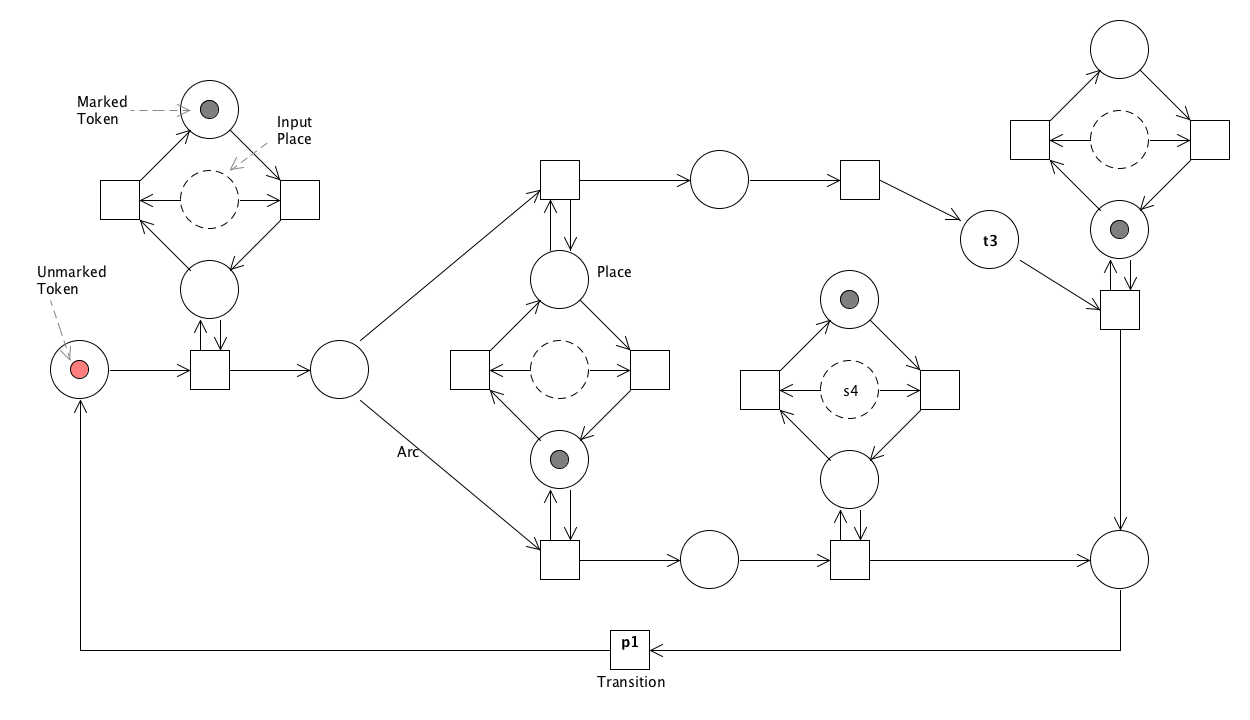
\includegraphics[scale=0.35]{image/petrinet_example.png}
		\caption{Petri net example}
		\label{fig:petrinet_example}
	\end{center}
\end{figure}

For the purpose of creating a 3D visualization of systems that can be modelled as a Petri net, the
application's user has to configure where the objects should be represented in the 3D space (and
this is what we called ''geometry'') and what the objects look like (''appearance''). Continuing our
example of the railway, for a proper visualization, the shape of the track has to be defined and the
positions of other elements (e.g. signals, switches) have to be fixed. An example of such a
configuration can be seen in Figure \ref{fig:geometry_example}.

\begin{figure}[htp]
	\begin{center}
		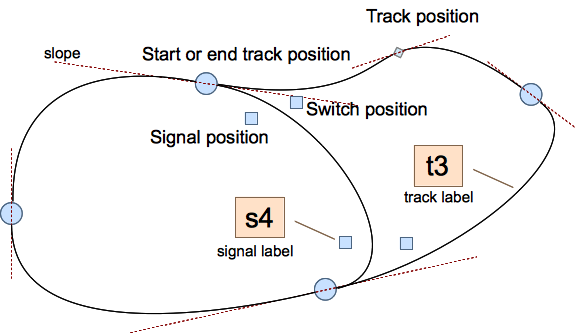
\includegraphics[scale=0.40]{image/geometry_example.png}
		\caption{Geometry example}
		\label{fig:geometry_example}
	\end{center}
\end{figure}

The ultimate goal of \epns is to visualize and interact with a dynamic system by using an
extended Petri net model enriched with features that will allow the user to correlate the model with
the physical world. Animation and visualization of an underlying Petri net model would constitute an
excellent feature that could potentially assist users in efficiently examining and analyzing the
model.

The following actors have been identified:

\begin{description}
    \item[the technical user] - has knowledge of Petri nets and uses the software
    to design the networks according to the desired specifications.
	\item[the non-technical user] -doesn't know the specifics of Petri nets, but needs to see the
	simulation of a discrete system, so he can have a better understanding of the real-life system.
	This type of user will only use pre-existing Petri nets (could be Petri nets created by the first
	type of user), with the required additional configurations, and run the simulation.
\end{description}

The following case is used to prove the utility of the project in a practical scenario. An engineer
could use this tool to design the extended Petri net, assigning any possible attributes to it (such
as shape and identity), so as to include any possible characteristics of the physical 3D objects he
might want to visualize. After the completion of the Petri net configuration, this technical user
could couple the underlying model with a 3D-animation to present it to his manager. The manager does
not need to have any understanding of Petri nets, but he can still evaluate the model and get a
clear view of its internal functionality.

From the user's point of view, the system can be divided in three parts:

\begin{description}
	\item[the Petri net and Animation Editor] - where a user (the technical user)
	sets the design of the Petri net, the animation associated with each place and
	the appearance of a token.
	\item[the Geometry Editor] - where a (technical) user sets the geometry of the
	system; for the railway example, in the geometry editor, the user sets the
	shape, length and appearance of the railway.
	\item[the Simulator] - where both types of users can see a 3D representation
	of the modeled system.
\end{description}

All the components and the way they interact with one another will be thoroughly described in the
following sections.

\subsection{Basic functionality}
\writer{Cosmin}
In order to use \epns, the application user starts by using the \textbf{Petri net Editor} to create
and configure the Petri net and the \textbf{Animations} that are executed during the simulation.
These will be later loaded by the \textbf{Graphical Simulator}, which, after being started, will
simulate the movement of tokens through the Petri net and will execute the configured animations,
resulting a visual representation of the Petri net's simulation on the screen.

Then, using the \textbf{GeometryEditor}, the \textbf{Geometry} would be created. It would be later
used by the \textbf{Graphical Simulator} in order to know how (on which paths) to move objects/token
representations and where to place different objects in the 3D space\footnote{Even though the
geometry is specified in a 2D space, during the simulation, all the object representations will be
drawn as 3D objects moving on a plane.}.

The \textbf{Graphical Simulator} also requires information about the \textbf{Appearance}, in order
to know how to represent tokens, tracks and other objects during the simulation. It is a simple
editor that connects labels (keys) with 3D Models(vrml, png, jpg \ldots), textures or just plain
data (Colors, Shapes).
  
The last step is to create a \textbf{Configurator} that connects the previously created
configurations and allows the user to start the graphical simulation. When started, the
\textbf{Graphical Simulator} reads the state of the simulation from the \textit{Petri net}. This read
state does not include exact positions of tokens in space, this information being loaded from the
\textit{Geometry}, or appearance information, loaded from the \textit{Appearance}. After
initialization, the Graphical Simulator displays the state of the simulation and handles all the
users' interaction as specified in the rest of this document.

For further details of what exactly each of the components allows the users to do please check the
following section or, in order to get more details regarding how to use \epns, please read the
\textit{Handbook}.

\subsection{General concepts}
\writer{Cosmin}
\label{oa:generalconcepts}
This subsection will introduce the general concepts used in the \epns system. More details will be
provided in the~\nameref{sec:architecture} and~\nameref{sec:system_features} sections, however the
most important concepts are presented below.

First of all, the classical concepts of \textbf{Petri nets} have been extended to accommodate the
required information for the graphical visualization of the simulation:
\index{Petri net} 
\begin{description}
\index{Petri net!Input Place}
\item[Input Places] - in order to provide the users with more power and customizability, some of the
Places in the Petri net can be configured to allow users, during the graphical simulation, to drop
(create) tokens. These are called \textit{Input Places} and act as normal Places in all other
respects, except for that they permit the possibility of a token being created there. For example,
in a train track simmulation, it allows the creation of simulation features such as a Traffic lights
or switches with which the users can interact during the graphical simulation.
\index{animation}
\item[Animations] - can be associated by the user to a particular Place and are run when a Token is
added on that Place, either by result of executing a transition or by being dropped there (after a
user interaction). Even though the token is removed from the source Places of the fired Transition,
they are not available for firing a new Transition until the animations associated with a place are
finished. More details will be specified later, but the supported animation types include: moving an
object on a path, showing or hiding objects, wait a fixed amount of time.
\item[Place Appearance] - each Place can have an associated appearance, describing how it must look
like in the Graphical Simulator.
\item[Token Appearance] - each Token can have an associated appearance, describing how it must look
like in the Graphical Simulator. Thus, the appearance of a Token will not change based on a place.
This will allow multiple tokens, with different representations, to be on the same place/track.
\item[Arc Identities] - each arc can have attached an identity used to control the flow of tokens
(or, more precisely, of token representations) in the simulation. For e.g., if we have a Transition
with one input Arc and two output Arcs and we take the case of simulating a train running on a
track, using the same identity on the input Arc and on one of the ouput Arcs will tell the Graphical
Simulator to move the Token representation (a train), which came on the input Arc, on the
corresponding output Arc. This allows a token representation to move continously in the direction
the user wants, without being destroyed or unnecessarily recreated.
\end{description}

Regarding the \textbf{Geometry}, as defined, it allow the users to specify the positions of objects
and the paths on which they move in the simulation space. The most important related concepts that
need to be presented at this point are:
\index{geometry}
\begin{description}
\index{Petri net!Track}
\item[Track] - defines how a curve (or line), on which an animation can take place, looks like. It
can also be connected with information about what the surface of this track looks like and usually
are used as graphical representations of Places.
\index{Petri net!Simple Position}
\item[Simple Position] - defines just a position in the simulation space and can be connected to the
an appearance it has. Can be used for completing the specification of some animations, for
representing an Input Place or just for displaying simple objects during the simulation.
\end{description}

Referring to the \textbf{Appearance}, it allow the users to easily define how objects look like
during the simulation. In \epns, there are mainly two big types of appearances that can be
configured:
\index{appearance}
\begin{description}
\item[Shape] - defines how a 3D Object displayed in the simulation should look like. For example, it
can be a reference to a file storing a 3D Model, which can then be loaded in the application or it
can simply be a 3D Object, such as a Cube or Sphere.
\item[Surface] - defines how a surface displayed in the simulation should look like. It can be
applied, for example, to a train track, and it could be either just a Color or a reference to a file
containing a texture that can be applied on the surface.
\end{description}



\section{System Features}
\label{sec:system_features}
\writer{Juan}

In this section we will start by presenting a general overview of the software being developed, 
showing its main components and how they will interact with the user, as well as with each other. 
Afterwards, we will go into more detail in order to find out what part each component will play 
during the execution of the program, describing the various functionalities each one will or may provide. 
Specific use cases showing the interaction between each component and the users are also provided, 
showing how they can be used and what is offered to the users.

\begin{figure}[htp]
\begin{center}
  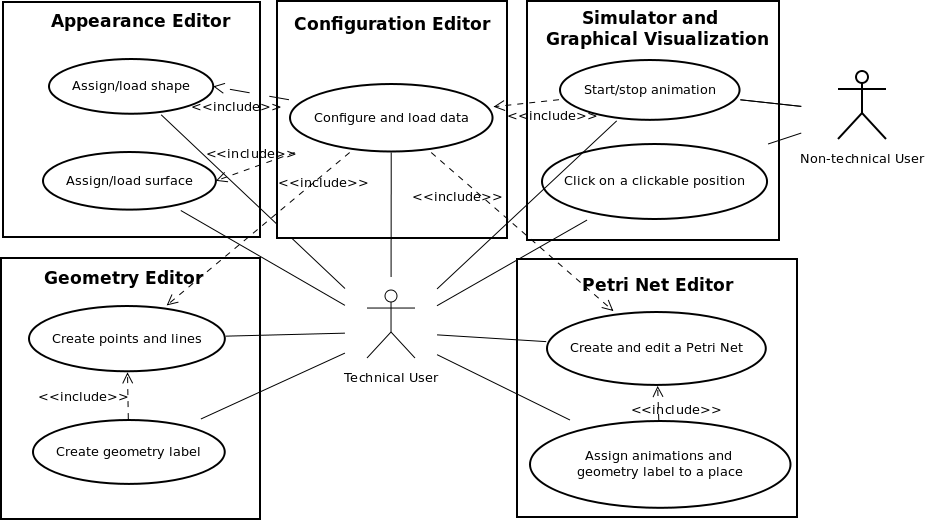
\includegraphics[scale=0.5]{image/uc_general.png}
  \caption{System Use Cases}
  \label{fig:system_use_cases}
\end{center}
\end{figure}

In Figure~\ref{fig:system_use_cases} we can see the manner in which the different components of the software in
development interact with each other and in what way they use one another. External to the software are 
the technical and non-technical user, who are given a set of functionalities to work with. As we can see, 
the technical user will be making use of the editors to set up everything that is needed for the Petri net simulation/visualization. He/She (or any 
non-technical user) will then be able to view the simulation thanks to the Simulator and Graphical 
Visualization component.

\subsection{Petri net Editor}
\index{Petri net!Editor}
\writer{Pablo}

This component will extend the ePNK tool to provide new features to the user, 
such as Input Places. It will also include the Animation Editor, which provides the user with a way of 
creating and configurating the animations for the Petri net that will be simulated. The user will be able 
to assign different Animations to be executed when Tokens reach different Places of the Petri net with this functionality.

\subsubsection{Functional requirements}

\begin{enumerate}
  \item The Petri net editor \textbf{shall} allow the user to create and edit Places.
  \item The Petri net editor \textbf{shall} allow the user to create and edit Transitions.
  \item The Petri net editor \textbf{shall} allow the user to create and edit Arcs to connect Places and Transitions.
  \item The Petri net editor \textbf{shall} allow the user to create and edit Tokens inside Places.
  \item The Petri net editor \textbf{shall} allow the user to create and edit Input Places.
  \item The Petri net editor \textbf{shall} allow the user to assign and edit Labels to the objects created.
  \item The Petri net editor \textbf{shall} allow the user to assign Animations to Places of the Petri net.
  \item The Petri net editor \textbf{shall} create a Petri net and Animation Configuration file that can be read by the Simulator.
  \item The Petri net editor \textbf{shall} allow the user to define a Sequence of Animations.
  \item The Petri net editor \textbf{shall} establish a relationship between a defined Geometry and a Place in the Petri net.
  \item The Petri net editor \textbf{shall} allow the user to save Petri net models.
  \item The Petri net editor \textbf{shall} allow the user to load existing models.
  \item It \textbf{would be nice} to allow the user to save a Sequence of Animations specifying a name for it to use it whenever he or she wants.
  \item It \textbf{would be nice} to give the user a preview of a defined Animation.
\end{enumerate}

\subsubsection{Use Cases}
\index{Petri net!Use cases}
See Figure~\ref{fig:petrinet_use_cases} for the Petri net Editor's use cases. The main features of this editor are shown, specifying the
functionalities provided by our system to allow 3D visualization.

\begin{figure}[htp]
\begin{center}
  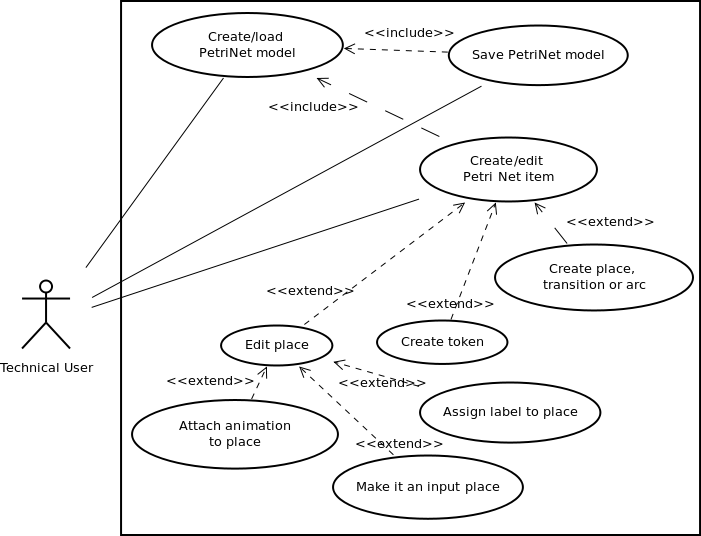
\includegraphics[scale=0.5]{image/uc_petrinet.png}
  \caption{Petri net Use Cases}
  \label{fig:petrinet_use_cases}
\end{center}
\end{figure}

\subsection{Geometry editor}
\index{Geometry!Editor}
\writer{Juan}

This component allows users to create a Geometry for the designed Petri net. It will allow him/her to define a 
Geometry for the Places of said Petri net.

\subsubsection{Functional requirements}

\begin{enumerate}
  \item The Geometry Editor \textbf{shall} allow the user to create points.
  \item The Geometry Editor \textbf{shall} allow the user to create lines connecting two points.    
  \item The Geometry Editor \textbf{shall} create a Geometry Configuration file that can be read by the configurator.
  \item The Geometry Editor \textbf{shall} allow the user to establish a relationship between a Geometry item and 
  its Appearance from the Appearance Configuration.
  \item The Geometry Editor \textbf{should} allow the user to create curves defined by a limited number of intermediate points.
  \item The Geometry Editor \textbf{shall} allow the user to load a Geometry Configuration.
  \item The Geometry Editor \textbf{shall} allow the user to save a Geometry Configuration.
  \item It \textbf{would be nice} to allow the user to create curves defined by any number of intermediate points.
  \item It \textbf{would be nice} to provide a history of the previous actions performed during the current editing process (for Redos, Undos...).
  \item It \textbf{would be nice} to provide the user a set of predefined figures like circunferences or squares.
  \item It \textbf{would be nice} to allow the user to save figures.
  \item It \textbf{would be nice} to allow the user to assign different lengths to the figures added in order to represent real proportions.
\end{enumerate}

\subsubsection{Use Cases}
\index{Geometry!Use cases}

See Figure~\ref{fig:geometry_use_cases} for the Geometry Editor's use cases.

\begin{figure}[htp]
\begin{center}
  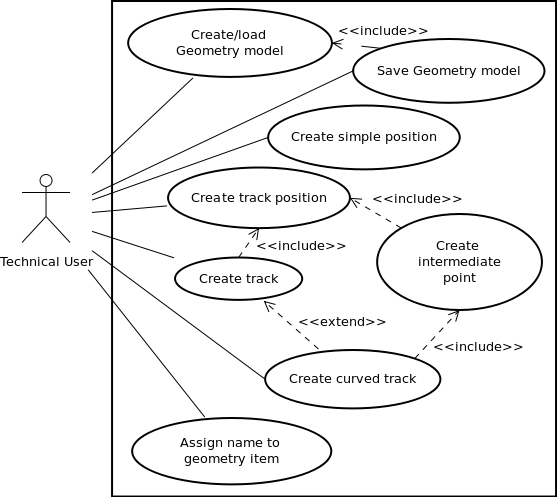
\includegraphics[scale=0.5]{image/uc_geometry.png}
  \caption{Geometry Use Cases}
  \label{fig:geometry_use_cases}
\end{center}
\end{figure}

\subsection{Appearance editor}
\index{Appearance editor}
\writer{Juan}

This component allows the user to set the shape and surface of the objects
belonging to the visual representation of the Petri net to be simulated.

\subsubsection{Functional requirements}

\begin{enumerate}
  \item The Appearance Editor \textbf{shall} allow the user to create 3D objects by choosing a predefined simple shape.
  \item The Appearance Editor \textbf{shall} allow the user to create surfaces by choosing a predefined color.
  \item The Appearance Editor \textbf{shall} create an Appearance Configuration file that can be read by the Configurator.
  \item The Appearance Editor \textbf{shall} allow the user load an Appearance Configuration.
  \item The Appearance Editor \textbf{shall} allow the user to save an Appearance Configuration.
  \item The Appearance Editor \textbf{should} allow the user to create 3D objects by referencing an existing 3D model.
  \item The Appearance Editor \textbf{should} allow the user to create surfaces by referencing an existing texture.
  \item The Appearance Editor \textbf{should} allow the user to assign a surface to a 3D object.
  \item It \textbf{would be nice} to provide the user with a collection of pre-defined complex shapes.
  \item It \textbf{would be nice} to allow the user to choose the colour from a palette.
\end{enumerate}

\subsubsection{Use Cases}
\index{Appearance editor!Use cases}

See Figure~\ref{fig:appearance_use_cases} for the Appearance Editor's use cases.

\begin{figure}[htp]
\begin{center}
  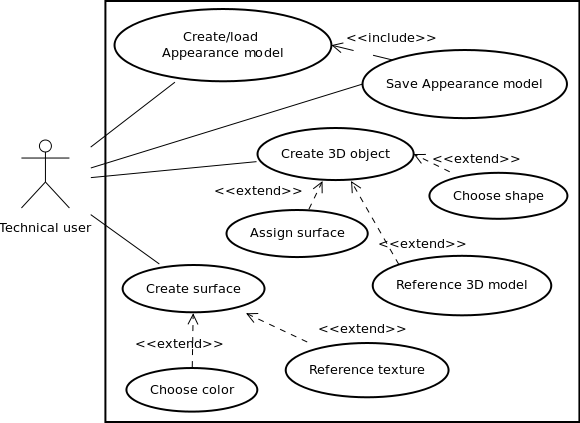
\includegraphics[scale=0.5]{image/uc_appearance.png}
  \caption{Appearance Use Cases}
  \label{fig:appearance_use_cases}
\end{center}
\end{figure}

\subsection{Configuration Editor}
\index{Configuration editor}
\writer{Juan}

This component allows the user to configure a simulation, by connecting the Petri
Net, Geometry and Appearance files used in the simulation and visualization.

\subsubsection{Functional requirements}

\begin{enumerate}
  \item The Configuration Editor \textbf{shall} allow the user to set a reference to the file containing the Petri net and Animations Configuration.
  \item The Configuration Editor \textbf{shall} allow the user to set a reference to the file containing the Geometry.
  \item The Configuration Editor \textbf{shall} allow the user to set a reference to the file containing the Appearance.
  \item The Configuration Editor \textbf{shall} allow the user to start the visualization of the simulation with the configured data.
  \item It \textbf{would be nice} to allow the user to set some aditional attributes that are not related to a concrete editor 
  (e.g. default track width or background color).
  \item It \textbf{would be nice} if, once the Petri net is loaded, the Geometry and Appearance Configurations are detected automatically based on name and extension.
\end{enumerate}

\subsubsection{Use Cases}
\index{Configuration editor!Use Cases}

See Figure~\ref{fig:configuration_use_cases} for the Configuration Editor's use cases.

\begin{figure}[htp]
\begin{center}
  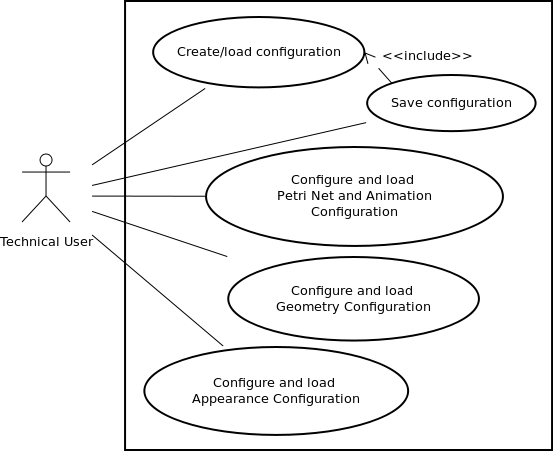
\includegraphics[scale=0.5]{image/uc_configurator.png}
  \caption{Configuration Use Cases}
  \label{fig:configuration_use_cases}
\end{center}
\end{figure}

\newpage
\subsection{Simulation and Graphical visualization tool}
\writer{María}

This component simulates the behaviour of the Petri net and provides a 3D
visualization of the objects defined for it, as well as the corresponding animations.

\subsubsection{Functional requirements}

\begin{enumerate}
  \item The graphical visualization functionality \textbf{shall} show a 3D visualization of the Geometry defined in the Geometry Configuration.
  \item The graphical visualization functionality \textbf{shall} show a 3D visualization of the Animations.
  \item The graphical visualization functionality \textbf{shall} detect when a user interacts with the visualization, i.e. clicks on a clickable position.
  \item The graphical visualization functionality \textbf{shall} allow the user to start/stop the animation.
  \item The graphical visualization functionality \textbf{should} allow the user to pause/restart the animation.
  \item The simulation functionality \textbf{shall} simulate the given Petri net.
  \item The simulation functionality \textbf{shall} allow the user to start as many simulations of the same Petri net as he or she wants.  
  \item It \textbf{would be nice} to load a Petri net at initialization and allow the user to edit it in parallel without interfering with the simulation.
  \item It \textbf{would be nice} to offer a visualization of the changes in the Petri net during the simulation.
\end{enumerate}

\subsubsection{Use Cases}

See Figure~\ref{fig:simulation_use_cases} for the Simulation \& Graphical Visualization tool's use cases.

\begin{figure}[htp]
\begin{center}
  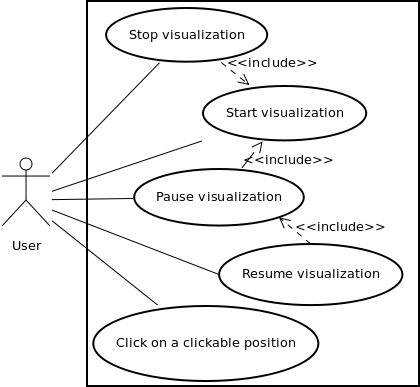
\includegraphics[scale=0.5]{image/uc_visualization.png}
  \caption{Simulation and Graphical Visualization Use Cases}
  \label{fig:simulation_use_cases}
\end{center}
\end{figure}



\section{Non-functional requirements}
\writer{María}

The purpose of this section is to specify a number of requirements that are not
related with the domain and analysis part. These requirements are divided in the three following subsections.

\subsection{Implementation constraints}

The system shall be implemented as a plug-in for the Eclipse framework version
Juno 4.2. It is a requirement to build the system using the following technologies/tools:

\begin{listliketab} 
  \storestyleof{itemize} 
  \begin{tabular}{Lll}
  	\textbullet & EMF - (Eclipse Modeling Framework) & v. 2.3.0 \\
  	\textbullet & GMF - (Graphical Modeling Framework) & v. 2.0.1 \\
  	\textbullet & ePNK & v. 0.9.4 \\
  	\textbullet & Java 3D & v. 1.5.1 
  \end{tabular} 
\end{listliketab}

\subsection{Documentation}

During the development process the following documents shall be delivered before
the specified deadline:

\begin{listliketab} 
  \storestyleof{itemize} 
  \begin{tabular}{Lll}
  	\textbullet & Project definition        & - 05/10/2012 \\
  	\textbullet & UML diagrams 		        & - 12/10/2012 \\
  	\textbullet & System specification 		& - 02/11/2012 \\
  	\textbullet & Draft version of handbook	& - 23/11/2012 \\
  	\textbullet & Final documentation		& - 21/12/2012
  \end{tabular} 
\end{listliketab}

\subsection{Code deliverables}

Some intermediate prototypes and experiments are required to be delivered:

\begin{listliketab} 
  \storestyleof{itemize} 
  \begin{tabular}{Lll}
  	\textbullet & Technology experiment 	 & - 26/10/2012 \\
  	\textbullet & First prototype 		     & - 16/11/2012 \\
  	\textbullet & Feature complete prototype & - 30/11/2012 \\
  	\textbullet & Final software 			 & - 21/12/2012
  \end{tabular} 
\end{listliketab}

\subsection{Quality}

In order to ensure the quality of the product, a set of procedures have been
established. These procedures are different depending on whether a document or a piece of code is being developed.

\subsubsection{Quality of documentation measures}

\begin{enumerate}
  \item Before starting to write a new document, some members of the group shall define the main structure and the 
  number of people working on each part. Afterwards, a brief explanation shall be done to the rest of the group.
  \item A first draft of the document should be ready at least a week before the deadline, so that all the members 
  of the group can read it and propose improvements.
  \item A final version of the document should be prepared at least two days before the deadline, so that all the 
  members of the group can check writing and consistencies.
  \item Once the document is approved, one member of the group shall be in charge of formatting it.
  \item One member of the group shall be in charge of delivering it before the specified deadline.
  \item The document shall be changed and checked as described above based on the feedback received by the professor.
\end{enumerate}

\subsubsection{Quality of implementation measures}

\begin{enumerate}
  \item All implementations should be reviewed by at least two members of the group, so that errors can be minimized.
  \item Every version of the code shall be committed to the SVN repository, with a comment about the changes made.
  \item Each component should be tested by a member of the group that has not taken part in the implementation, to ensure that every possible scenario is covered. Unit testing should be used for this purpose when possible and acceptance testing when not.
  \item Integration tests shall be carried out in order to check the correct behaviour of each of the pieces connected.
  \item System tests shall also be used to check the correct behaviour of the whole product. 
  \item Every piece of code shall have comments explaining the steps, in order to allow the rest of the group to understand it. 
  \item It would be nice to create a programming style document before starting the implementation process.
  \item Javadoc shall be used to provided thorough documentation of the code.
\end{enumerate}

%%%%%%%%%%%%%%%%%%%%%%%%%%%%%%%%%%%%
%%%%%%%%%% USER INTERFACE %%%%%%%%%%
%%%%%%%%%%%%%%%%%%%%%%%%%%%%%%%%%%%%
\section{User interface}
\writer{Jerome}
This chapter describes the main aspects regarding how the User Interface of our Software product looks.

%%%%%%%%%% TECHNOLOGIES %%%%%%%%%%
\subsection{Technologies}
The GUI shall be implemented using Eclipse plugins. These plugins are of various types and together work to obtain the desired functionality. The used types are:

\begin{description}
  \item[Editor] - used for the creation and edition of the different resources (Resource Editor) to design the networks according to the desired specifications.
  \item[View] - show the different properties of the resource currently being edited (Diagram Overview).
  \item[Pop-up] - used to add extra functionalities (Right-click Menu).
\end{description}

%%%%%%%%%% GUI PARTS %%%%%%%%%%
\subsection{GUI parts}
In this section, we will talk in more details about all the different parts of the global editor running in Eclipse that will be provided with the software. Throughout this document we will refer to this as the Workbench. The Workbench is composed of five main parts as shown in Figure \ref{fig:gui_editors}: the Project Explorer, the Resource Editor, the Properties View, the Diagram Overview and finally the ToolBar.

The most important components are the Project Explorer, the Resource Editor and the Properties View because they allow the user to interact with the software, creating new parts or editing them. In the following sections a short description of all the different parts will be provided.

\begin{figure}[htp]
\begin{center}
  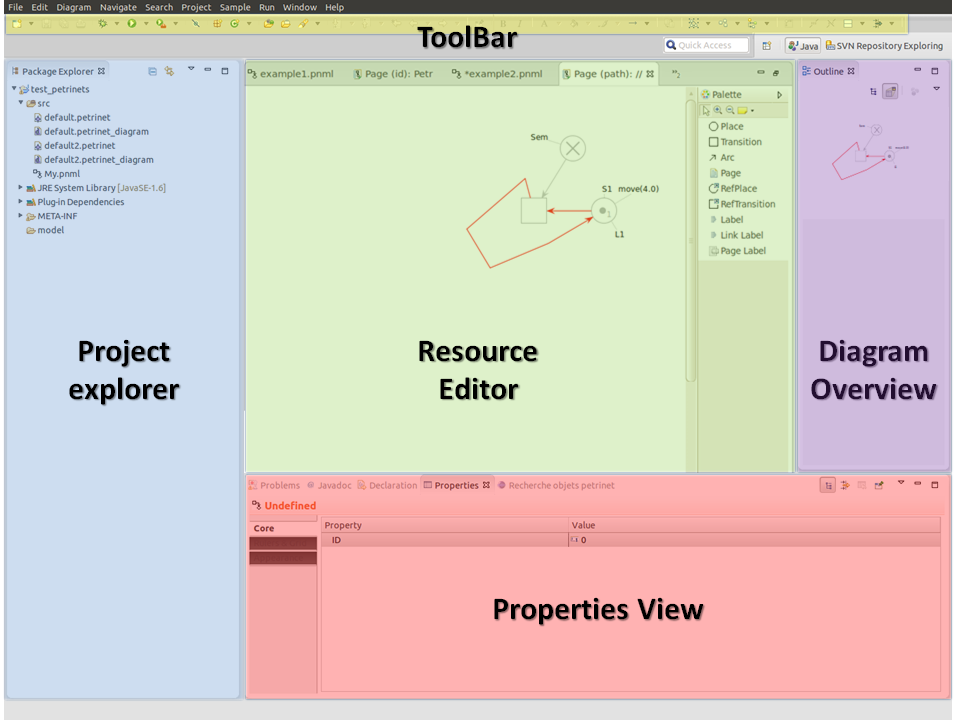
\includegraphics[scale=0.45]{image/gui_editors.png}
  \caption{Workbench}
  \label{fig:gui_editors}
\end{center}
\end{figure}

%%%%% Project Explorer %%%%%
\subsubsection{Project Explorer}
The Project Explorer is a standard Eclipse view. It provides the user with an overview of the project showing the different folders and files composing it, with their extensions. By selecting a file and pressing Enter, the view will determine what type of file the user has selected and open the Editor associated with this type of file (see Figure \ref{fig:gui_file_editor}).

\begin{figure}[htp]
\begin{center}
  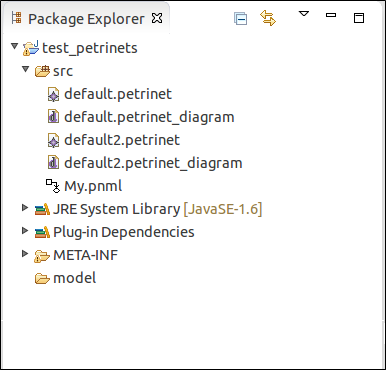
\includegraphics[scale=0.45]{image/gui_file_editor.png}
  \caption{Eclipse Project Explorer}
  \label{fig:gui_file_editor}
\end{center}
\end{figure}

%%%%% Resource Editor %%%%%
\subsubsection{Resource Editor}
This part of the Workbench is an Editor, more precisely a set of Editors. In the following figure you will see a representation of the Petri net Editor,
which allows the user to create, design and modify Petri nets. (See Figure \ref{fig:gui_petri_editor}).

\begin{figure}[htp]
\begin{center}
  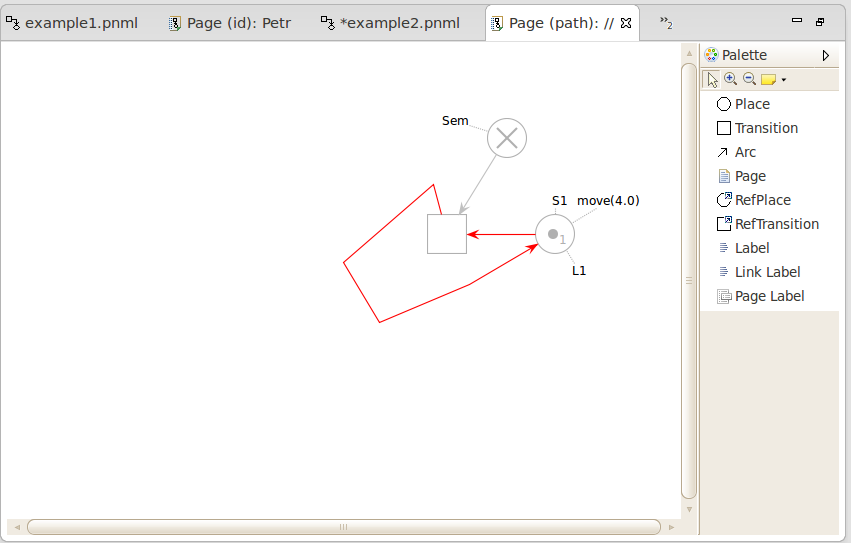
\includegraphics[scale=0.45]{image/gui_petrinet.png}
  \caption{Petri net Editor}
  \label{fig:gui_petri_editor}
\end{center}
\end{figure}

The Resource Editor is split into two parts : the left area contains a graphical representation of the resource the user is editing while the right area displays a
Palette of elements that the user can drag and drop to modify the graphical part.

In the graphical representation, the user is allowed to move elements, resize them and edit their name by double-clicking on them. The Palette contains some other useful tools such as zooming and adding notes in the graphical representation so the user can explain to another user some parts of his representation. In addition to the Petri net Editor, we also have three other Editors provided with our software: the Geometry Editor that allows the user to draw a shape (for example, the shape of the track) that will be associated with the Petri net for the simulation (See Figure \ref{fig:gui_geometry_editor}); the Appearance Editor that provides a way to edit the appearance of Places and Tokens; and the Configuration Editor that keeps a reference to the Petri net Model and the Geometry Model to configure the simulation.

\begin{figure}[htp]
\begin{center}
  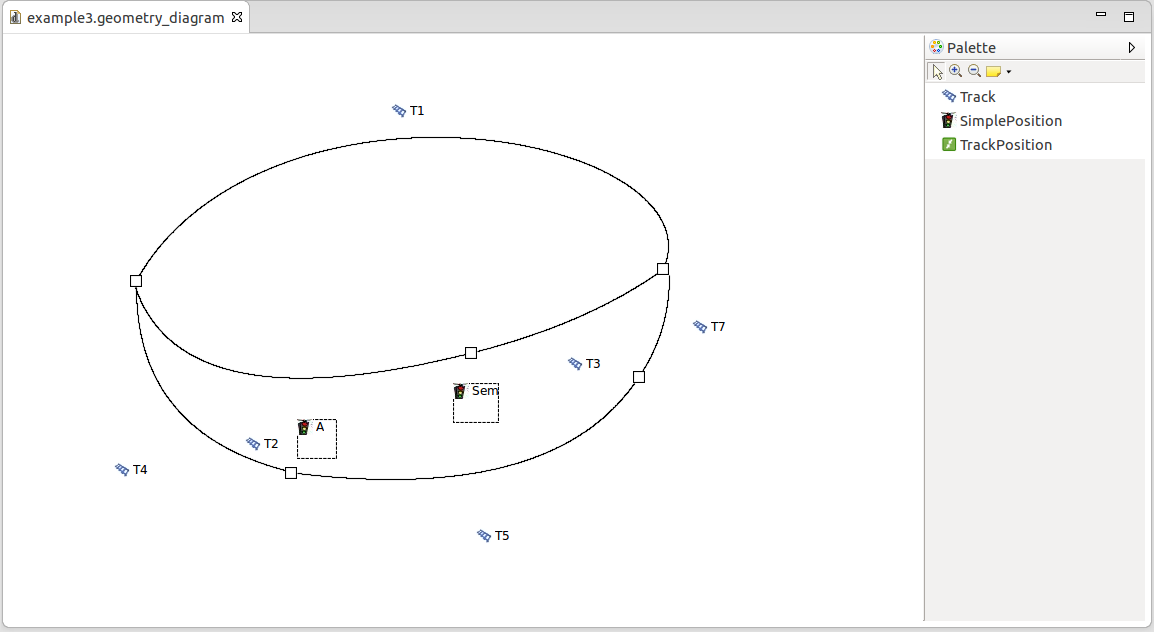
\includegraphics[scale=0.45]{image/gui_geometry_editor.png}
  \caption{Geometry Editor}
  \label{fig:gui_geometry_editor}
\end{center}
\end{figure}

%%%%% Properties View %%%%%
\subsubsection{Properties View}
The Properties View is another one Eclipse built-in plugin displayed as a view. This view is connected to the Resource Editor and displays some additional properties depending on the selected object. The goal of the Properties View is to edit the properties of different objects of the diagram. The Figure \ref{fig:gui_property_editor} below will for example provide you the Properties View associated with the selection of a Transition in our Petri net editor.

\begin{figure}[htp]
\begin{center}
  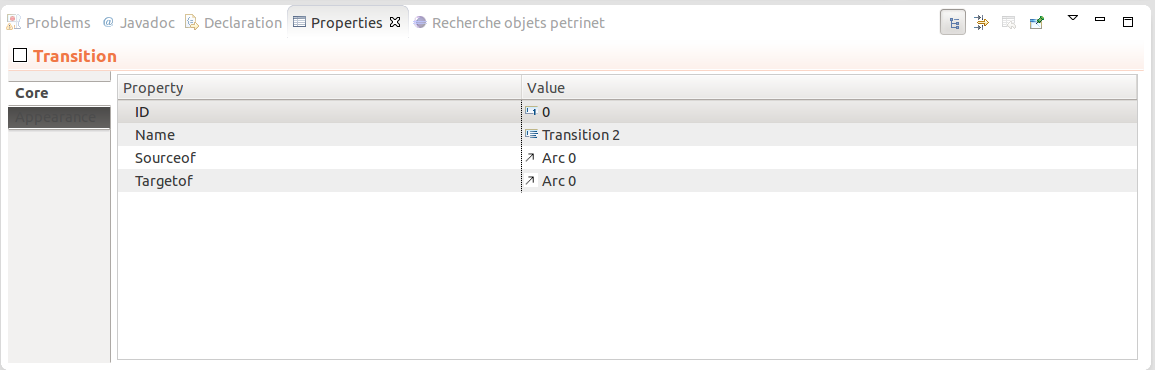
\includegraphics[scale=0.30]{image/gui_property_editor.png}
  \caption{Property View}
  \label{fig:gui_property_editor}
\end{center}
\end{figure}

%%%%% Diagram Overview %%%%%
\subsubsection{Diagram Overview}
One more useful Eclipse plugin is the Diagram Overview, also implemented as a view. The particularity of this view is that its goal is to show a global view of the Diagram we are editing with a box symbolizing the part we are actually seeing in the Resource Editor. As a diagram can be a lot bigger than the user's screen this plugin is used to navigate through the Diagram as the Resource Editor will display what is inside the box and we can move the ``seeing box'' dragging it in the Diagram Overview (see Figure \ref{fig:gui_diagram_overview}).

\begin{figure}[htp]
\begin{center}
  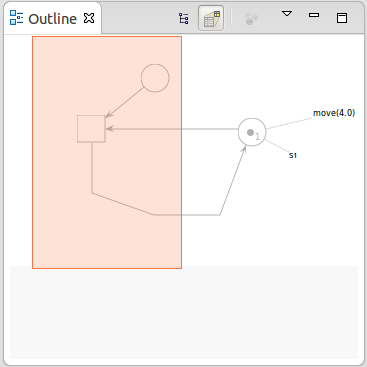
\includegraphics[scale=0.50]{image/gui_diagram_overview.png}
  \caption{Seeing box}
  \label{fig:gui_diagram_overview}
\end{center}
\end{figure}

%%%%% Tool Bar %%%%%
\subsubsection{ToolBar}
The ToolBar is the area in Eclipse where all the general functions are placed. This includes commands like creating, saving and loading, next and previous page, etc (see Figure \ref{fig:gui_toolbar}).

\begin{figure}[htp]
\begin{center}
  
\includegraphics[scale=0.40]{image/gui_toolbar.png}
  \caption{Toolbar}
  \label{fig:gui_toolbar}
\end{center}
\end{figure}

%%%%% Right Click Meny %%%%%
\subsubsection{Right-click Menu}
This global menu (in the sense it can be accessed everywhere) is not shown in our Figure \ref{fig:gui_editors}. It can be triggered by the user pressing the right button of his mouse. It will show some relevant options such as delete object, or start some actions. Indeed each content of the menu will depend of the type of selected component. As an example, we can show the "Start Simulation" action that has been implemented in \epns. This function is only available when a right-click is performed on a ``Configurator'' object and allows launching of the Simulation and the Visualization for the Petri net  (see Figure \ref{fig:gui_popup_menu}).

\begin{figure}[htp]
\begin{center}
  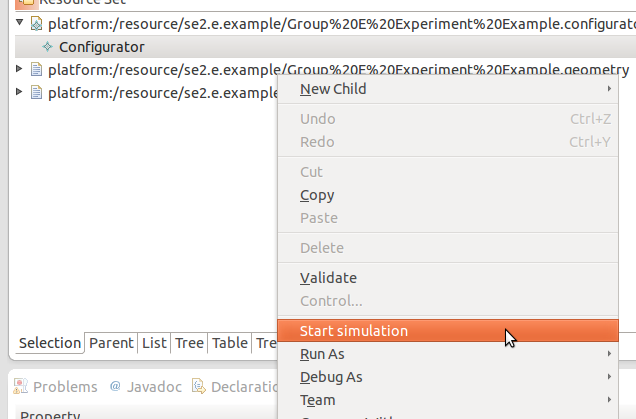
\includegraphics[scale=0.40]{image/gui_popup_menu.png}
  \caption{Right-click Menu}
  \label{fig:gui_popup_menu}
\end{center}
\end{figure}

%%%%% Simulator %%%%%
\subsubsection{Simulator and Graphical Visualization}
\index{Simulator!UI}
This last component is also not shown in Figure~\ref{fig:gui_editors} as it is a window detached
from Eclipse. It provides a 3D visualisation of a chosen Petri net using the Geometry Model and the
Appearance Model that have been set up earlier. It has two main buttons: Start/Stop and Pause/Resume
allowing the user to control the simulation \& visualization. The user may also interact with the
tool by clicking on the interactive input places in the simulator to trigger events, for example to
change the status of a a traffic light from the red to the green state (see Figure
\ref{fig:gui_simulator}).

\begin{figure}[htp]
\begin{center}
  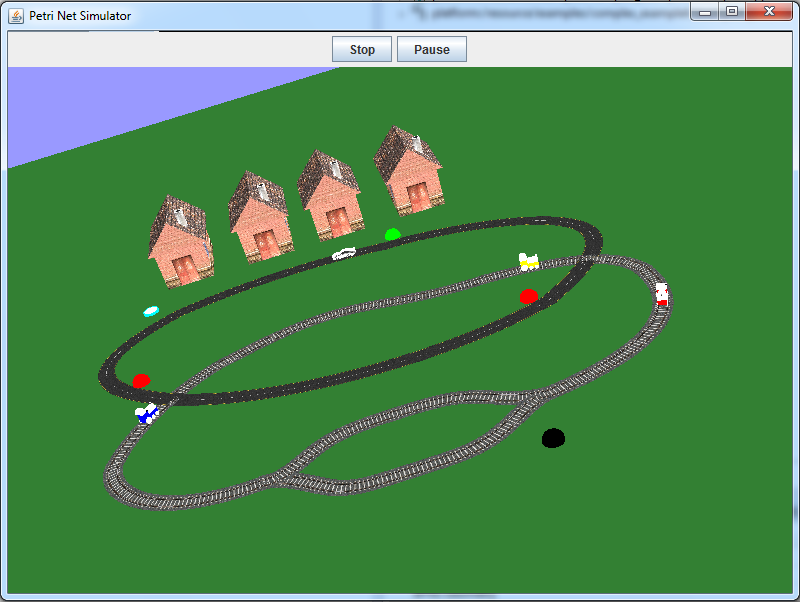
\includegraphics[scale=0.50]{image/gui_simulator.png}
  \caption{The Simulator}
  \label{fig:gui_simulator}
\end{center}
\end{figure}

\section{Architecture}
\writer{Cosmin, Ruxandra, Anders - Intro Part}
\label{sec:architecture}

The overall architecture is based on the principle of modularity.
The system is separated in several components, with well defined
interfaces. This approach has several advantages:
\begin{itemize}
  \item The development of components can be easily delegated to different group
    members. As long as the interfaces remain the same, changes can be made to the
	component behind that interface with minimum influence on other components.
  \item Components can be easily tested
  \item Due to the interfaces, components can easily be mocked, therefore making it 
  	possible to test the overall system in a structured manner. 
\end{itemize}

\begin{figure}[ht]
   \begin{center}
       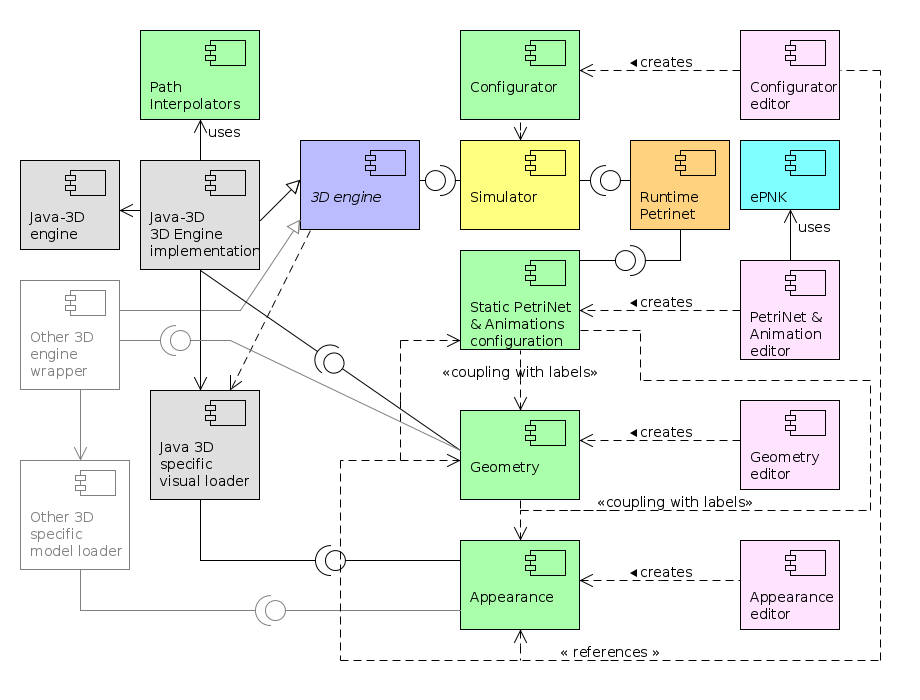
\includegraphics[scale=0.35]{image/components.png}
       \caption{Components diagram}
       \label{fig:components}	
       \end{center}
   \end{figure}

A general view of the domain model is presented in figure \ref{fig:components}. A short description of 
the most important components will be provided in the next paragraphs. More details are available
in the sections dedicated to each component. 

In order to use our system, the application user begin by using the \textbf{Petri net Editor}
to create the \textbf{Static Petri net}. When starting the \textbf{Simulator}, it would load
the \textbf{Static Petri net} and create a \textbf{Runtime Petri net}. This runtime Petri net
contains the information about Places, Arcs and Transitions, but also contains up-to-date information 
regarding the tokens present in each Place(a hash-map).

The way the tracks look like is defined in the \textbf{Geometry editor}. The settings from the geometry 
editor will be used by the 3D Engine in order to know how (on which paths) to move objects/tokens when instructed by the
Simulator. This \textbf{Geometry editor} allows the usee to create paths (curves) in the 3D space, which will
be used when animating objects during the simulation. Moreover, it allows the user to add positions on
which to place various objects(like traffic lights, trees, etc.) in the 3D space.

The 3D Engine also requires information about how the objects will look like, in order
to know how to represent tokens, tracks and other objects during the simulation. This information is set up in 
the \textbf{Appearance editor}.It is a simple editor that connects labels with 3D Models(.3ds and .obj), 
3D Shapes, Textures or Colors.

For setting up animations for the objects in the simulation we will use an \textbf{Animation Editor},
which, in our project is integrated in the Petri net editor to create an easier and more intuitive 
interface for the user. The user can set up a single animation or a sequence of animations which is
loaded by the Simator and is then used by the 3D engine to display the objects.

The \textbf{Simulator} is a component that supports the simulation of a Petri net.
In order to do so, the Simulator needs a \textbf{Petri net} to simulate, a
\textbf{3D engine} to display the simulation on and the settings provided by the \textbf{Geometry editor}, 
\textbf{Appearance editor} and the integrated \textbf{Animation Editor} to know how to map
Petri net concepts to 3D coordinates.

The \textbf{3D engine} is an abstraction of 3D engines with focus of Petri net simulations of
objects on tracks (see project definition). The idea is to facilitate various 3D engines: Java3D,
OpenGL, HTML5 without having to reimplement everything. Our system will make use of an abstract factory for
the wrapper implementations and their 3D models.

\begin{figure}[ht]
   \begin{center}
       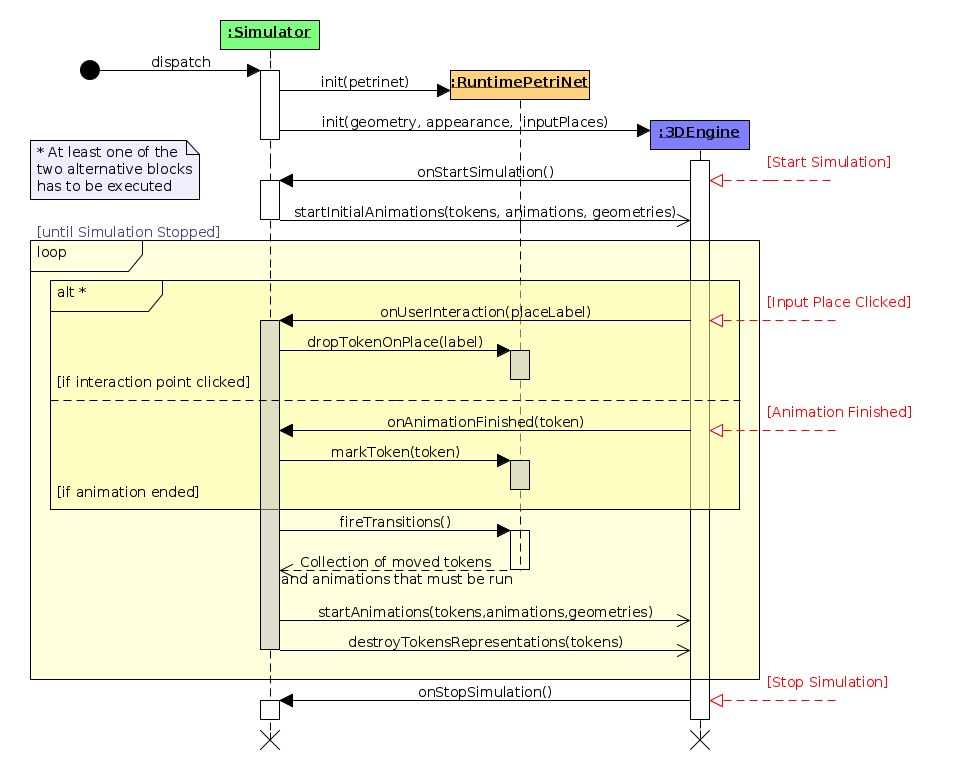
\includegraphics[scale=0.50]{image/system_sequence_diagram.png}
       \caption{System Sequence Diagram}
       \label{fig_ssd}
       \end{center}
   \end{figure}

In Figure~\ref{fig_ssd}, we represented the interaction between the main components active during a
running simulation \& visualization. The Simulator is the main component, which is started by the
user and has access to all the configuration files necessary. Then, the 3D engine is started by sending
the Geometry and Appearance configurations and the Input Places. Next, the Runtime Petri net is
initialized based on the static Petri net created by the technical user. The actual simulation is started
by the user, by clicking the Start button, event which is captured by the 3D Engine. 
The latter notifies the Simulator that the simulation was started, which, in turn, starts the
initial animations.

The simulation runs in a loop where animations are started for tokens on places. Whenever
an animation ends, the 3D Engine notifies the Simulator and the corresponding token in the Petri net
is marked as finished. If an interactive input Place has been activated (clicked upon the associated 3D Object),
then a token is created in it. In either case, the RuntimePetriNet is asked to fire any waiting
transitions \footnote{Considerations should be made on infinite loops by the technical user
configuring the network.}. A collection of moved tokens and the animations that have to be run is
returned. Using this, the Simulator might need to start new animations or to destroy representation
for tokens that do not exist in the simulation anymore\footnote{More details will be provided in
subsequent sections.}. Then the loop starts over.

The simulation stops when a special place (e.g. a Stop button) is pressed in the 3DEngine, which, in
turn, notifies the 3D Engine accordingly.

In the rest of this chapter, more details are provided for each of the components used in \epns
and general implementation details are discussed.

\subsection{Petri net Editor}
\writer{Pablo}

\index{Petri net}
\index{Petri net!Editor}
As previously stated, this component is logically separated into two parts: the Petri
net Editor itself (see figure \ref{fig:petrinet_domain_model}) and the Animation Editor
(see figure \ref{fig:animation_domain_model}). Therefore, we will describe them separately.

\index{Petri net!Domain model}
\begin{figure}[ht]
   \begin{center}
       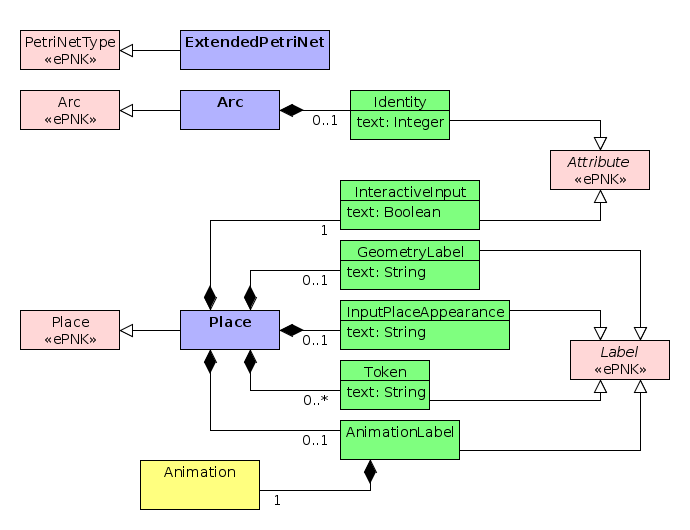
\includegraphics[scale=0.50]{image/dm_petrinet.png}
       \caption{Petri net Domain Model}
       \label{fig:petrinet_domain_model}
   \end{center}
\end{figure}

\subsubsection{ePNS Petri net classes}
\label{lst:pn_classes}
Here are described the classes that define the components of an ePNS Petri
net according to the model used for the software in development (the model is shown in
figure \ref{fig:petrinet_domain_model}).

\newpage
\textbf{Arc class} \\
The Arc class has the following attributes:
\begin{description}[labelindent=1cm]
  \item[Identity:] an ePNK Attribute with an integer that indicates the Arc's identity (used
for Token flow, for more information see "Arc Identities" in \ref{oa:generalconcepts}).
\end{description}

An Arc connects Places to Transitions and vice versa, as well as determining (thanks to
their Identity attribute) which way Tokens must go when "going through" Transitions.

\textbf{Place class} \\
The Place class has the following attributes:
\begin{description}[labelindent=1cm]
  \item[InteractiveInput:] an ePNK Attribute with a boolean value indicating whether Tokens
can be inserted into the Place (for more information see "Input Place" in \ref{oa:generalconcepts}).
  \item[GeometryLabel:] an ePNK Label with a string containing the name of the Geometry object
that will represent the Place (this will typically be a line or a point in the geometrical
description; for more information see "Track" and "SimplePosition" in \ref{arch:geometryeditor}).
  \item[InputPlaceAppearance:] an ePNK Label with a string containing the name of theAappearance
of the Place (only used if the Place is an Input Place, for more information see "Place Appearance"
in \ref{oa:generalconcepts}).
  \item[Token:] an ePNK Label representing a token with a string indicating the name of the
Appearance that will be associated to said token (for more information, see
"Token Appearance" in \ref{oa:generalconcepts}). As in classic Petri nets, a Place may contain any number of Tokens.
  \item[AnimationLabel:] an ePNK Label containing an Animation object (this will indicate the
Animation or Animation Sequence to be executed on a Token that is inserted into the Place,
whether this is through a Transition or through external means; for more information on Animations,
see "Animations" in \ref{oa:generalconcepts}).
\end{description}


\subsubsection{Animation classes}
\index{Petri net!Animation Editor}

Here are described the classes that define the animations of the
components of an ePNS Petri net for the later visualization.

\begin{figure}[ht]
   \begin{center}
       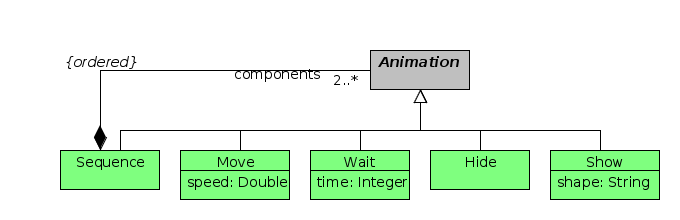
\includegraphics[scale=0.50]{image/dm_animation.png}
       \caption{Animations Domain Model}
       \label{fig:animation_domain_model}
   \end{center}
\end{figure}
  
\textbf{Animation class}

The Animation class is a definition of an animation, which will be indirectly associated to different elements of the Geometry of the Petri net and the Appearance of its components. An Animation in itself isn't anything, the classes described below are the ones that specify an Animation's behaviour.

\textbf{Sequence class}

The Sequence class is an Animation object containing:
\begin{description}[labelindent=1cm]
  \item[components]: a set of 2 or more Animation objects
\end{description}

This class is used to model an aggregation of Animations.

\textbf{Move class}

The Move class is an Animation object containing:
\begin{description}[labelindent=1cm]
  \item[speed]: Real
\end{description}

A Move object represents an animation of an object moving at a certain speed along a Track that represents the Place to which the Animation is associated.

\textbf{Wait class}

The Wait class is an Animation object containing:
\begin{description}[labelindent=1cm]
  \item[time]: Integer
\end{description}

A Wait object models an animation in which an object waits for a certain amount of time (e.g., a car waits in a crossroads for 3000 miliseconds before entering it).

\textbf{Hide class}

This object models an ``animation'' where any object currently associated to the Place to which the Animation is applied is hidden from the screen.

\textbf{Show class}

The Show class is an Animation object containing:

\begin{description}[labelindent=1cm]
  \item[shape]: String
\end{description}

This class represents the ``animation'' of showing an object (described by its shape) in the position of the Place associated to this Animation (if the Place is represented by a Track the object will be shown at the beginning of the Track). This could be used to, for example, put a traffic light into the simulation in the following way:

\begin{enumerate}
  \item Two places are created, both with the same geometrical position. One of them has attached a show(green\_light) and the other a 
  show(red\_light), where green\_light and red\_light are the appearances of a green traffic light and a red traffic light respectively.
  \item When a Token moves into one of the Places, a traffic light (a green light in one of them and a red light in the other one) would be shown.
  \item An Input Place or a Wait Animation could be used to change from a green to a red traffic light.
\end{enumerate}

%%%%%%%%%%% GEOMETRY EDITOR %%%%%%%%%%%
\subsection{Geometry editor}
\writer{Georgios}
\label{arch:geometryeditor}
The Geometry Editor is the component with which the technical user will draw the geometry on which the Petri net behavior will be simulated. This will be achieved by providing a Geometry Model that basically describes what a Geometry object is comprised of, or in other words, what the components that make up a Geometry object are.

%The technical user is the appropriate one to provide the Geometry model to the Graphical Modelling Framework (GMF). Then, the GMF will autogenerate an editor, along with other code, on which the technical user will be able to draw different geometry object, such as lines and control points. GMF is based on the Model-View-Controller (MVC) architecture and it is a core technology of the final product that the Geometry Editor will utilize.

%Figure \ref{fig:geometry_editor_structure} shows the structure of a Geometry Editor.

%\begin{figure}[ht]
%   \begin{center}
%       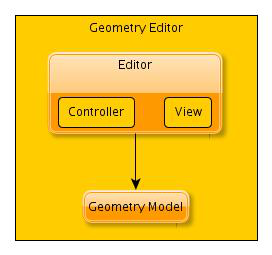
\includegraphics[scale=0.50]{image/geometry_editor_structure.png}
%       \caption{Geometry Editor Structure}
%       \label{fig:geometry_editor_structure}
%       \end{center}
%   \end{figure}

At this point the reader should recall that the simulation is track-bound. Thus, through the Geometry Editor the technical user will draw the paths (straight or curved lines-tracks) along which 3D objects will move. Furthermore, the technical user will have the possibility to set control points, such as a signals, with which the animation of the 3D objects could be controlled. Other than that, the Geometry Editor will allow for naming different geometry objects, such as tracks and signal positions. This could be achieved by a label attribute associated with every Geometry object. It constitutes a unique identifier for such an object. In this way the label attribute plays the role of one-to-one link between Places in the Perti Net and the Geometry objects. 

In particular, for visualising systems modeled as Petri nets in a track-bound manner, the Geometry model in Figure \ref{fig:geometry_domain_model} has been created.

\begin{figure}[ht]
   \begin{center}
       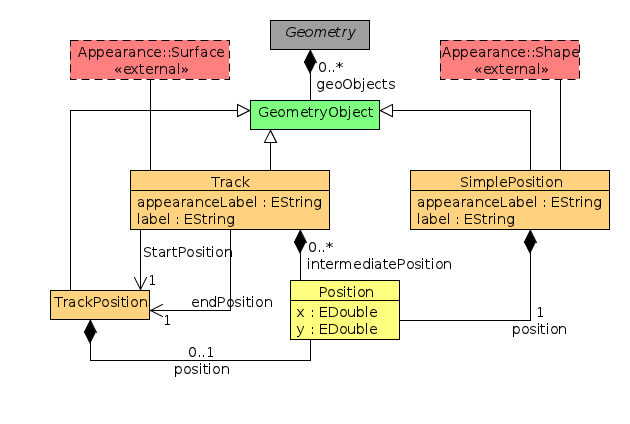
\includegraphics[scale=0.50]{image/geometry_domain_model.png}
       \caption{Geometry Domain Model}
       \label{fig:geometry_domain_model}
       \end{center}
   \end{figure}

A detailed description of each and every class in the model will be presented in that point. 

\textbf{Geometry}

The Geometry class is simply an abstract definition of a geometry. 

\textbf{GeometryObject}

The GeometryObject class is an empty class from which different geometry objects, such as Track, TrackPosition and SimplePosition, inherit. 

\textbf{Track}

A Track class consists of :
\begin{description}[labelindent=1cm]
  \item[appearanceLabel]: EString
  \item[label]: EString
\end{description}

A Track object resembles a line in the geometry. This line can be drawn between two TrackPosition objects. A Track can be either a straight or a curved line. A Track label constitutes a reference to that particular Track object while the appearanceLabel defines the appearance of the Track on hte 3D visualization space. 

\textbf{TrackPosition}

A TrackPosition is a GeometryObject that simply represents a point on a geometry. Two TrackPosition objects are needed for a Track to be created.

\textbf{Position}

A Position class contains :

\begin{description}[labelindent=1cm]
  \item[x]: EDouble
  \item[y]: EDouble
\end{description}

A Position object resembles a point in the two dimension space in a geometry. 

\textbf{SimplePosition}

A SimplePosition is a GeometryObject containing : 

\begin{description}[labelindent=1cm]
  \item[appearanceLabel]: EString
  \item[label]: EString
\end{description}

A SimplePosition object is correlated to one Position object. Its appearanceLabel defines the appearance of the SimplePosition object on the 3D visualaization space, while the label is a reference to it. 


%%%%%%%%%%% APPEARANCE EDITOR %%%%%%%%%%%
\subsection{Appearance Editor}
\index{Appearance Editor}
\writer{Jerome}
The Appearance Editor is another component we will provide to the user, allowing him to associate a visual representation to certain elements of the Petri net so each element can have a representation in the Simulator. This Editor should be used by the technical user and will be displayed as a tree. Each element of the tree will have a Label to identify it and some special properties to customize it.

We can see in Figure \ref{fig:appearance_domain_model}, the domain model associated to that component.

\begin{figure}[ht]
   \begin{center}
       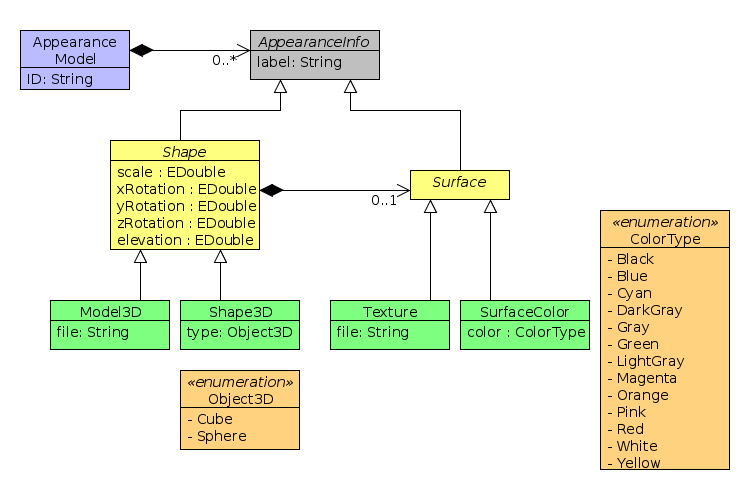
\includegraphics[scale=0.50]{image/dm_appearance.png}
       \caption{Appearance Domain Model}
       \label{fig:appearance_domain_model}
   \end{center}
\end{figure}

We will now describe in details each class of this domain model.

\textbf{Appearance Model}

The AppearanceModel class is simply an abstract definition of an appearance object. 

\textbf{AppearanceInfo}

The AppearanceInfo class is an empty class from which different appearance objects, such as Shape or Surface, inherit. 

\textbf{Shape}

A Shape class consists of :
\begin{description}[labelindent=1cm]
  \item[scale]: EDouble
  \item[xRotation]: EDouble
  \item[yRotation]: EDouble
  \item[zRotation]: EDouble
  \item[elevation]: EDouble
\end{description}

A Shape object that will be used for 3D elements. It has a lot of attributes such as scale that represents the scale the 3D object should be represented with, (x,y,z)Rotation that represent the rotation on each axe we have to apply for this object and elevation that represents the ``high'' the object has to be from the ground. This is also an abstract class and it can be inherited by the Model3D and Shape3D classes.

\textbf{Model3D}

A Model3D class consists of : 
\begin{description}[labelindent=1cm]
  \item[file]: String
\end{description}

A Model3D object contains a single proper attribute : file that represents the place of the 3D model file on the hard disk. It inherits from Shape.

\textbf{Shape3D}

A Shape3D class consists of : 
\begin{description}[labelindent=1cm]
  \item[type]: Object3D
\end{description}

A Shape3D object contains a single proper attribute : type that represents the type of 3D shape we want to load. These types are already configured internally and don't use any external 3D shape. This class inherits from Shape.

\textbf{Object3D}

An Object3D enumeration consists of :
\begin{description}[labelindent=1cm]
  \item[Cube]
  \item[Sphere]
\end{description}

An Object3D is a pre-configured 3D shape that can be used for our software. If the user wants to have another 3D shape he needs to use the Model3D object.

\textbf{Surface}

A Surface class is simply an abstract definition of a 2D object. It can be inherited from the Texture and SurfaceColor classes.

\textbf{Texture}

A Texture class consists of : 
\begin{description}[labelindent=1cm]
  \item[file]: String
\end{description}

A texture object contains a single proper attribute : file that represents the place of the Texture of the Surface on the hard disk. It inherits from Surface.

\textbf{SurfaceColor}

A SurfaceColor class consists of : 
\begin{description}[labelindent=1cm]
  \item[color]: ColorType
\end{description}

A SurfaceColor object contains a single proper attribute : color that represents the color of the Surface. This color will be one color we have pre-loadedin our software. The list of all different colors is the enumeration ColorType. This class inherits from Surface.

\textbf{ColorType}

A ColorType enumeration consists of :
\begin{description}[labelindent=1cm]
  \item[Black]
  \item[Blue]
  \item[Cyan]
  \item[DarkGray]
  \item[Gray]
  \item[Green]
  \item[LightGray]
  \item[Magenta]
  \item[Orange]
  \item[Pink]
  \item[Red]
  \item[White]
  \item[Yellow]
\end{description}

A ColorType is a pre-configured color we can use for coloring a Surface.
 
%%%%%%%%%%% CONFIGURATION EDITOR %%%%%%%%%%%
\subsection{Configuration Editor}
\writer{Ruxandra}
The Configuration Editor consists of only one class that links the Petri net,
its Geometry and its Appearance. In order to link them, the Configurator class
contains references to each of the previously mentioned classes. Also, the Configurator contains an attribute specifying the width of all the tracks in the scene. A simple
diagram that describes how the configurator gathers all the information needed
for the running simulation is shown in Figure~\ref{fig:configuration_dependencies}.

\begin{figure}[ht]
   \begin{center}
       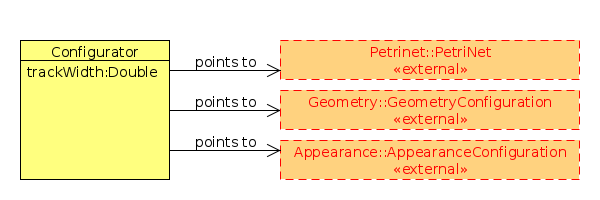
\includegraphics[scale=0.50]{image/configuration_dependencies.png}
       \caption{Configuration Dependencies}
       \label{fig:configuration_dependencies}
       \end{center}
   \end{figure}

After editing all the files, linking them in the Configurator file and setting the track width, the
simulation can be started by pressing ``Start simulator'' in the pop-up menu when right-clicking the configurator object.

\subsection{Simulator}
\index{Simulator}
\writer{Ruxandra, Marius}
The Simulator is the mediator between the RuntimePetriNet and the 3DEngine. At the initialization, it receives all the necessary data to start the simulation and the 3D visualization: the Petri net model, its geometry, its appearance and the animations associated. The simulator processes
the information received, creates a RuntimePetriNet and initializes the 3D engine with the
geometry, the appearance and the animations. It then waits for the user's input (press start button) to start the animations for the  initial tokens. The way the 3D engine and the RuntimePetriNet work will
be discussed in the next sections.

As it can be seen in figure \ref{fig:simulator_design}, the simulator implements the Engine3DListener
interface which means that it listens to the 3Dengine: it is notified when the
user start the simulation, when an animation is finished, when the user clicks
on a interactive input point or when the user stops the simulation. In each
case, it takes the appropriate measures to produce the required response.

\begin{figure}[ht]
   \begin{center}
       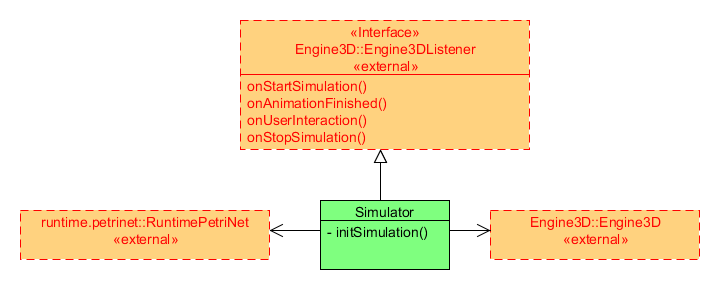
\includegraphics[scale=0.50]{image/simulator_design.png}
       \caption{Simulator with listener}
       \label{fig:simulator_design}
       \end{center}
   \end{figure}

\subsection{RuntimePetriNet}
\index{RuntimePetriNet}
\writer{Ruxandra}
The RuntimePetriNet is the component that knows where a Token is located in
the Petri net at each step of the simulation. It can be noticed that the Token
from the static Petri net is replaced in the RuntimePetriNet by a RuntimeToken,
while the Places and Transitions classes are the same. The reason for this decision
is that the places and transitions are neither created nor deleted during the
simulation(i.e. they are static components), unlike tokens, which are created
and deleted at each execution of a transition. Therefore, tokens need to be
small objects, containing just the relevant information, not all the irrelevant
information (irrelevant for the actual simulation) inherited from EMF objects.

Figure \ref{fig:petrinet_references} shows the internal structure of the RuntimePetriNet. It provides
five public methods that can be called from other classes (in our case from the
Simulator): init(), which initializes the RuntimePetriNet's structures and returns the 
movements(defined by a token and the place where the token is created) for the inital tokens; fireTransitions(), 
which iterates over all the transitions from the Petri net and executes all the ones that can be executed; fireTransition(), which
executes only one transition and returns information about the new places of tokens after executing thay transition;
markToken(), which is called whenever an animation finishes and a token needs to
be marked as finished (in order to allow previous animations to finish); getInputPlaces() which returns all
the geometry labels for the places that are defined as input places(see \ref{lst:pn_classes})

\begin{figure}[ht]
   \begin{center}
       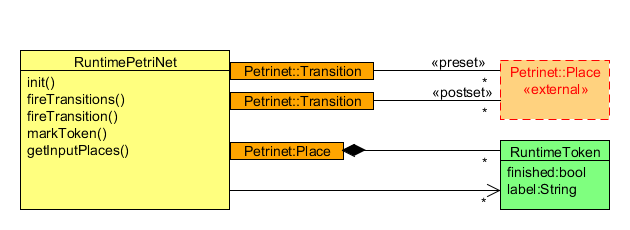
\includegraphics[scale=0.50]{image/runtime_petrinet.png}
       \caption{Runtime Petri net}
       \label{fig:petrinet_references}
       \end{center}
   \end{figure}

Structurally, the RuntimePetriNet has a dictionary that associates a place with
all the RuntimeTokens it contains, whether they are marked or not. It can be
seen in figure \ref{fig:petrinet_references} that a RuntimeToken has two main attributes : one is for
checking if the corresponding animation has finished and one for indicating the
way the RuntimeToken will look in the 3D visualization. The RuntimePetriNet
contains also two optimizations for rapidly retrieving the presets and postset
of a transition : a dictionary that associates each transition with all the
places in its preset and a dictionary that associates a transition with all the
places in its postset.

\subsection{3D Engine}
\index{3D Engine}
\writer{Cosmin}

The 3D Engine is the component of the application that handles the drawing and animation of the
objects from the simulation, on the screen. It's main responsibilities include:

\begin{itemize} 
  \item the handling of the Window in which the graphical simulation takes place
  \item handling of the buttons through which the user can interact with the simulation (Play,
  Pause, Stop)
  \item drawing the representations for the objects in the graphical visualization
  \item maintaining an association between the 3D Objects that represent the elements from the Petri
  Net and the actual Petri net objects (Tokens, Places)
  \item updating the animations according to the configurations
  \item handling user input in the case of Input Places
\end{itemize}

In order to build a system that can be easily modified, the interaction between the Simulator and
the 3D Engine is done by employing Interfaces and the Factory and Observer patterns. This
interaction can be seen in the Figure \ref{fig:engine_relations}.

\begin{figure}[ht]
   \begin{center}
       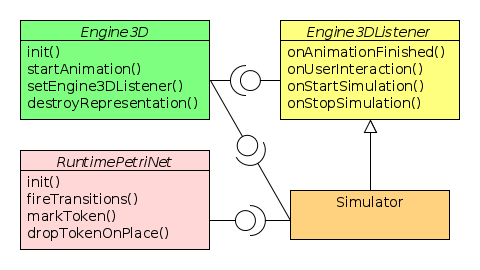
\includegraphics[scale=0.50]{image/engine_relations.png}
       \caption{3D Engine Interactions}
       \label{fig:engine_relations}
       \end{center}
   \end{figure}

The Simulator is the one that uses the Engine3DFactory to get a reference to an implementation of
the Engine3D. Then, it initializes the Engine by providing it the configurations for the Geometry
and the Appearance and registers itself as an Engine3DListener. The Engine3D keeps a reference to an
Engine3DListener (in our implementation this is the Simulator) and for every event that can occur
(e.g. an animation is finished, an user interaction has been detected, the animation was started or
stopped) it notifies it. During a normal run, when an animation is finished or an user interaction
has been detected the Engine3D notifies the Simulator using the Listener's interface and, in return,
the Simulator uses the Engine3D interface to start required animations.

Figure \ref{fig:engine_structure} shows a detailed view of \epns's implementation for the Engine3D
Interface presented above. Java 3D was chosen as the supporting 3D framework. We will now shortly
describe each of the components in the diagram and their interaction.
 
\begin{figure}[ht]
   \begin{center}
       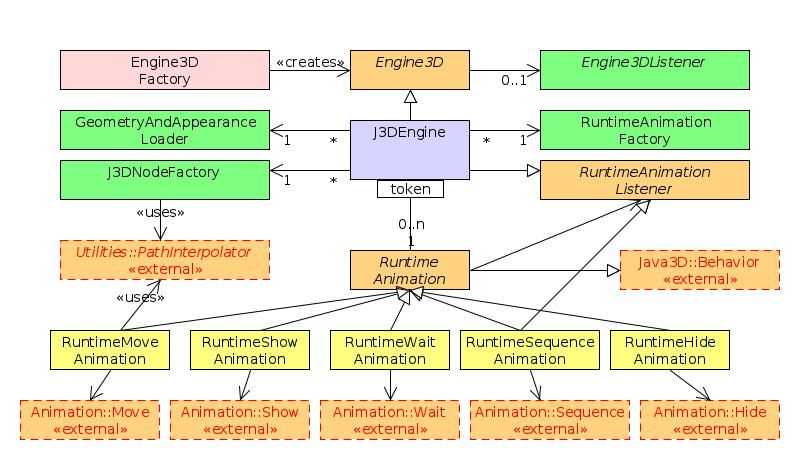
\includegraphics[scale=0.50]{image/engine_structure.png}
       \caption{3D Engine}
       \label{fig:engine_structure}
       \end{center}
   \end{figure}
   
\textbf{J3DEngine} - This class is the core implementation for our Engine3D and is handling the main
logic for the graphical representation of the simulation. Besides this, it interacts with the
Simulator, either by receiving calls (through the methods defined in the Engine3D interface) or by
sending notifications to it (through the Engine3DListener interface). Also, this class takes care of
initializing the Java 3D environment and the Window and handles user interaction.

\textbf{Engine3DListener} - As mentioned before, this is used to allow a proper mechanism for the
Engine3D to notify interested components of events regarding the simulation. As it can be seen in
Figure~\ref{fig:engine_relations}, such a listener has to implement 4 methods which allows it to be
notified when the user starts the simulation, when an animation is finished, when the user clicks on
a interactive input place or when the user stops the simulation. Using it allows the 3D Engine to
work independently of other components. For example, the J3DEngine could also be used by something
else besides the Simulator, for the purpose of animating objects.

\textbf{GeometryAndAppearanceLoader} - This helper class is initialized by the J3DEngine with the
Geometry and Appearance configurations. It loads the necessary data (e.g. textures, models etc.)
and, when required by the engine, serves geometry or appearance information.

\textbf{J3DNodeFactory} - The node factory is a Java3D dependent class, that handles the building of
the various Java3D nodes and branches, for different representations of the objects during the
visualisation. Basically, given the geometry or appearance label, it creates a new Java3D node (or
alters an existing one, if required) used for displaying objects according to the user's
preferences. For example, these nodes are used to display Token representations, visualization for
Geometry \textit{Tracks} or \textit{Simple Positions}. For the purpose of creating the tracks'
representations, the \textit{PathInterpolator} is used to compute where(position) / how(rotation)
quads should be placed to obtain a proper display result.

\index{3D Engine!Runtime Animations}
\textbf{RuntimeAnimation} - This abstract class is used by the J3DEngine to manage the animations
that are running. It holds all the required information (e.g. the RuntimeToken it is animating,
references to Java3D Nodes in the scene graph etc.). It is built as a unit that completely
self-manages its life-cycle: after it is initialized and started, all the required actions / updates
are performed automatically by it and the finalization actions \& notifications are executed
accordingly, without any other operations performed by other component (e.g. J3DEngine, Simulator).
In order to properly implement this, the Java3D \textbf{Behaviors} are used, the RuntimeAnimation
abstract class actually being an extension of the \textit{Behavior} class. What it does it that it
attaches itself to the Java3D scene graph and, based on the implementing classes (one for each
Animation - see below), it sets up wakeup conditions in order to execute code exactly when needed
(e.g. at every \textit{X} frames, after a time interval has passed etc.)

\textbf{RuntimeAnimationListener} - This interface allows the RuntimeAnimations to communicate with
other classes interested in the progress of \textbf{RuntimeAnimation}s. To exemplify, for the simple
Animations (Move, Wait, Show and Hide), the J3DEngine is used as a listener, so it is informed, for
example, when the animations are finished. However, the Sequence Animation also implements this
interface and, when executed, starts the 'child' animations by itself and registers itself as a
listener for them. Thus, when one of the animations in the sequence is finished, the next one is
started. The Sequence Animation also has to handle the proper forwarding of wakeup conditions
between the child animations and the Java 3D Engine.

\textbf{RuntimeMoveAnimation, RuntimeSequenceAnimation, RuntimeWaitAnimation, RuntimeShowAnimation,
RuntimeHideAnimation} - These 5 classes are implementations of the \textbf{RuntimeAnimation}
interface presented above and each of them takes into consideration the particularities of the
Animation type it refers to. They employ Java3D features to display the required animation or to
have the desired effects. Considering that most of the control logic is implemented in the
\textbf{RuntimeAnimation} class, these implementation mostly have to focus on the actions needed to
be performed and the next moment when they should execute actions again (see
Table~\ref{tab:runtime_animation}).

\begin{table}[ht] \centering
    \begin{tabular}{| l || l | l | } 
		\hline
		\textbf{Implementation} & \textbf{Actions} & \textbf{Next Wakeup} \\
		\hline
		Move Animation & Move the token representations & Fixed framerate \\
		Wait Animation & Just wait & Set up time interval \\
		Show Animation & Show the object & Never \\
		Hide Animation & Hide the object & Never \\
		Sequence Animation & Initialize animations and forward wakeups & When child animations require \\
		\hline
	\end{tabular}
	\caption{Table showing Runtime Animations actions and wakeups}
	\label{tab:runtime_animation}
\end{table}

\textbf{RuntimeAnimationFactory} - This class is used as a Factory class in order to initialize the
implementation for the \textbf{RuntimeAnimation} corresponding to a given \textbf{Animation}.

\subsection{Path Interpolators}
\writer{Anders}

In order to make paths in the geometry editor and their counterparts in the simulator look the same,
a utility component has been developed. As it is an architectural choice, that the simulator should
be open for new implementations of the 3D engine, it was crucial that the path interpolator component
should be independent of both GMF, EMF, and of course the chosen 3D engine. Also, not knowing the 
choice of data types in alternative 3D engines, it was chosen use \texttt{double} as the base type
for coordinates, Carthesian and polar. Another choice could have been \texttt{BigDecimal}, but knowing that 
even \textbf{Open GL} only uses float, and that BigDecimal is inefficient because of its need for garbage collection,
\texttt{double} was chosen as a fair compromise.

The path interpolators shall support the geometry editor with a list of points, that can easily be 
converted to a \texttt{PointList} without actually knowing that class. They also shall support 3D engines,
with exact position and orientation of an object at any distance from the start of a path. The two
representations shall reflect each other, even though the geometry editor does not need orientations.

Consequently two utility classes have been created: A vector (\texttt{Vector2D}) class that holds coordinates
and methods for calculating with vectors, and another class holding a vector for position and a vector for orientation.
The name of the latter class is \texttt{Where}, a name that might be changed in a later version.

The facade classes and interfaces of the path interpolator component are:

\begin{description}
  \item[\texttt{PathInterpolator}] This is the interface for interpolators in this component. It defines methods for getting the
      length of the underlying path, finding the position and orientation at any distance from the path start. These methods are 
      ment for the 3D engine to calculate where objects should be and what way they should point. I also defines a method
  	for getting intermediate point, a pixel apart, for the geometry editor. 
  \item[\texttt{Vector2D}] This is the presentation of a 2D vector. It can be used to define a position or an orientation. It supports
    Carthesian and polar coordinates. It has been developed with efficiency in mind. Many methods aim to produce as
    few new objects as possible, when making calculations.
  \item[\texttt{Where}] Is mainly a position and an orientation, implemented with two \texttt{Vector2D} fields.
    Several convenience methods are provided. 
\end{description} 

The concrete classes that implements the \texttt{PathInterpolator} interface are:

\begin{description}
  \item[\texttt{LinearPathInterpolator}] This interpolator works with straight lines, and is mainly provided as the 
    first prototype, and for testing purposes. It has also worked as a proof of concept to the \texttt{PathInterpolator}
    interface and the other facade classes.
  \item[\texttt{QuadraticBezierPathInterpolator}] This interpolator works with quadratic Bézier curves, quadratic Bézier curves
    works with two end points and an intermediate point defining the tangents to the two other points. This interpolator assumes
    that any other point is a tangent target, all other points are intermediate start/end points. In the case with an even
    number of points the last line will be straight. The code for this interpolator is \textbf{highly} inspired from the
    code in \textbf{ePNK} and uses a recursive approach.
  \item[\texttt{BezierPathInterpolator}] This interpolator uses any number of intermediate points and uses Bernstein polinominals
  	to calculate actual positions, see \ref{sec:bezier-curves} \nameref{sec:bezier-curves}.
  \item[\texttt{BezierCurvePathInterpolator}] This is a cleaned up version of \texttt{BezierPathInterpolator}. It also provides
  	extra points showing the tangents of the end points for the geometry editor.
\end{description}

The component includes additional helper classes, that can be used for other other purposes, not only in the scope of Petri net
simulations and Bézier curves. The most important are:

\begin{description}
  \item[\texttt{BezierCurve}] The \texttt{BezierCurve} class is the foundation of the \texttt{BezierCurvePathInterpolator}.
  	It incapsulates a list of \texttt{Vector2D} points and calculates the value for any $t$ $0 \leq t \and t \leq 1$ of the
  	Bézier function. It also finds the distance between two such values, and the \texttt{Where} of a distance from start $t = 0$.
  \item[\texttt{ToolBox}] The tool box is a class with static methods as the \texttt{java.lang.Math} class.
    It has methods for calculating:
    \begin{itemize}
  		\item the power of a real (\texttt{double}) number to an integer exponent. A recursive algorith is used here to increase
  		  efficiency.
  		\item the binominal coefficient of n over k. This is used by \ldots
  		\item the value of a Bernstein base polynonimal. 
	\end{itemize} 
\end{description}

\subsubsection{Bézier Curves}
\label{sec:bezier-curves}
\writer{Anders}

The most commonly known Bézier curves are quadratic and cubic Bézier curves. Quadratic Bézier curves uses three points, a start
and an end point and one intermediate point. The intermediate point determines the outgoing angle of the curve from the starting
point and the ingoing angle to the end point. The cubic Bézier curve has two intermediate points, each of them determining the 
outgoing angle of the start point and the ingoing angle of the end point, further more the distance of the intermediate points
determine the detour of the curve from start to end. Even more intermediate points can determine the detour more and more precisely.
The number of points besides the starting point, determines the order $n$ of the curve. An order $n = 1$ is a straight line,
$n = 2$ is a quadratic curve, and $n = 3$ is a cubic Bézier curve.

\begin{figure}[htp]
\begin{center}
	  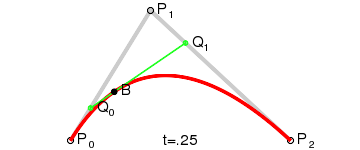
\includegraphics[scale=0.4]{image/wiki_bezier_2.png}
	  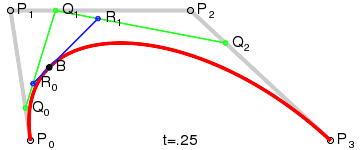
\includegraphics[scale=0.4]{image/wiki_bezier_3.png}
	  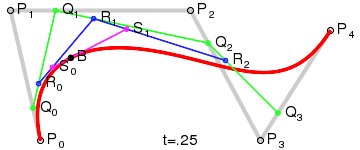
\includegraphics[scale=0.4]{image/wiki_bezier_4.png}
	  \caption{Bézier curves of order 2, 3, and 4}
	  \label{fig:wiki_bezier}
\end{center}
\end{figure}

Figure \ref{fig:wiki_bezier} shows Bézier curves of order two, three,
and four\footnote{The images has been borrowed from Wikipedia: http://en.wikipedia.org/wiki/Bézier\_curve}.
Most graphical programs doesn't use
more than third order (cubic) Bézier curves, and it is not recommended to add too many intermediate points
in the geometry editor, the curve will not be much nicer, but harder to calculate. 

In the component we use:

\begin{equation}
	B(t) = \sum_{i = 0}^n b_{i,n}(t)P_i
\end{equation}

wher $B(t)$ is the value of the Bézier function and $t \in [0,1]$. $b_{i,n}$ is the $i^{\text{th}}$ Bernstein polinomial of
degree $n$. $P_i$ is the $i^{\text{th}}$ intermediate point. The Bernstein polinomial is defined as follows:

\begin{equation}
	b_{i,n}(t) = \binom{n}{i}t^i(1-t)^{n-i}
\end{equation}

The binomial coefficient is calculated using this formula:

\begin{equation}
	\binom{n}{k} = \prod_{i = 1}^k \frac{n - k + i}{i}
\end{equation}

The implementations can be found in the \texttt{se2.e.utilities.ToolBox} class.

\section{Glossary}
\writer{Georgios}

\subsection{Technical Glossary}
\begin{description}
  \item[Animation] The dynamic behavior of objects on 3D Canvas that are associated with Places of the Petri Net model.
  \item[Appearance] The look and feel of the objects visualized by the 3DEngine .
  \item[Appearance Editor] A graphical editor provided EMF for configuring appearance.
  \item[Control GUI] A simple Graphical User Interface with appropriate actions (play/pause/stop buttons) so as the end user to be able to interact with the 3DEngine and consequently with underlying Petri Net execution .
  \item[Geometry] the track (3D line/curve) on which the 3D-visualization of the Petri Net simulation takes place. The geometry consists of predefined objects such as, semicircles, points and lines.
  \item[Geometry Editor] A graphical editor provided by ePNK and GMF for designing the area on which the simulation will be reflected.
  \item[Identity] The attribute of Arcs in the Petri Net model that defines the trajectory of the Tokens.
  \item[IgnoreAnimation] The attribute of Arcs in the Petri Net model that allows the target transition to fire without the associated Place Animation having finished.
  \item[Input place] a place in which tokens can be insterted externally, i.e. by clicking an interactive control point.
  \item[Interactive control point] A point that allows the user to interact with the system (e.g. by a click)
  \item[Petri Net Editor] A graphical editor provided by ePNK and GMF for designing the Petri Net of the system a user wants to visualize.
  \item[Physical object] A graphical object that is used by the 3DEngine for visualizing its behaviour during the Petri Net simulation.
  \item[Simulator] The software component that will provide the underlying Petri Net execution information to the 3DEngine so as to be able to visualize the Petri Net execution with 3D objects.
  \item[Shape] The visual traits of a physical object being part of the simulated system visualization.
  \item[Token] The Petri Net element that moves along Petri Net places through transitions.
\end{description}

\subsection{Technology Terms}
\begin{description}
\item[Ecore Tool editor] - The EMF editor that provides all the necessary elements for realizing or drawing the model in question.
\item[EMF] - The Eclipse Modeling Framework. It auto-generates code that represents the corresponding model (usually described in UML).
\item[EMF Validation Framework OCL Integration] -  Helps for expressing constraints on ambiguous graphical models such as a class diagram. Tightly used with UML users can define constraints on their models.
\item[ePNK] - The eclipse Petri Net  Kernel, a modern equivalent of PNVis missing the visualization part though. Built following the model-based software engineering paradigm. ePNK Petri Net Types to be extended to provide new functionality.
\item[GMF] - The Eclipse Graphical Modeling Framework provides the appropriate infrastructure for developing graphical editors based on EMF.
\item[Xtext] - Xtext is a framework for development of programming languages and domain specific languages.
\end{description}

\printindex

\end{document}

